\documentclass[a4paper,11pt,oneside]{book}

\author{Vincenzo Maffione}
\title{Optimization in Virtual Machine Networking}
\date{\today}

%\usepackage{syntonly}
%\syntaxonly

\usepackage{lmodern} 

\usepackage{amssymb} % simboli matematici AMS
\usepackage{amsmath}

\usepackage{txfonts}

\hyphenation{pro-prie-t� in-di-vi-duo re-le-ga-re mo-del-lo mo-del-li o-pe-ra-zio-ni o-pe-ra-to-ri mo-du-lo ri-ve-la-to per-met-te-re rap-pre-sen-ta-zio-ne mo-del-liz-za-zio-ne ge-ne-ra-to o-biet-ti-vo li-ne-a-re no-no-stan-te po-si-ti-va e-la-bo-ra-zio-ne o-pe-ra-ti-vo sca-la-bi-li-t� i-ni-zia-liz-za-re in-di-vi-duo o-pe-ra-to-re va-lo-ri i-te-ra-zio-ni in-va-li-da-re pe-ri-fe-ri-che re-gi-stri ma-na-ge-ment e-si-ste pra-ti-ca va-ria-bi-li in-di-riz-zo o-pe-ra-zio-ne me-dian-te in-di-vi-duo sem-pli-ci-t� co-lo-ri ha-mil-to-nia-no que-sta in-clu-de-re ge-ne-tic}


\usepackage[english]{babel}

%\usepackage{indentfirst} % indentazione nella prima riga di ogni capoverso

\setlength{\parindent}{0pt} % elimina l'indentazione sulla prima riga di ciascun capoverso


%\usepackage[T1]{fontenc} % migliora la sillabazione di lingue non inglesi
\usepackage[latin1]{inputenc} %codifica per le lingue latine


% definizione dell'ambiente "abstract", per aggiungere il sommario
\usepackage{fancyhdr}
\newcommand{\fncyblank}{\fancyhf{}}
\newenvironment{abstract}%
{\cleardoublepage\fncyblank\null\vfill\begin{center}%
\bfseries\abstractname\end{center}}%
{\vfill\null}

\usepackage{graphicx}

\linespread{1.3}  % aumenta l'interlinea di un fattore 1.3


\begin{document}

%\maketitle

\begin{titlepage}
\pagestyle{empty}
\begingroup
% intestazione
\vspace*{-8.5\topskip}

\begin{figure}[!h]
\begin{center}

\includegraphics[scale=0.3]{logo_sssup}
\end{center}
\end{figure}

\vspace*{-0.5cm}

\begin{center}
        \large{\bf\expandafter\textsc {Universit\'a di Pisa}}\par 
		  \large{\bf\expandafter\textsc {Facolt\'a di Ingegneria}}\par
		  \large{\bf\expandafter\textsc {Laurea magistrale in Ingegneria Informatica}}\par
        \vspace{0.5cm}
        \large{\bf\expandafter\textsc {Tesi di Laurea}}
\end{center}



% Titolo
\vspace{1.5cm}
\begin{center}
        {\LARGE\bf\textit{Optimization in Virtual Machine Networking}}
\end{center}

\vspace{1.5cm}



\begin{center}
\begin{tabular}{l p{3.3cm} r c}

\textsc{Relatore} & & \textsc{Il candidato} \\
&&\\
\dotfill&&\dotfill \\
Prof. \textit{Luigi Rizzo} & &\textit{Vincenzo Maffione}\\
{\small Universit\'a di Pisa} & &\\
 & &  \\
\textsc{Relatore} & &  \\
 \dotfill&&\\
Prof. \textit{Giuseppe Lettieri} && \\
{\small Universit\'a di Pisa} && \\
 & & \\

\end{tabular}
\end{center}

\vspace{0cm}


\begin{center}
Anno Accademico 2012-2013
\end{center}
\par
\vfill\par 
\clearpage
\endgroup
  

\end{titlepage}

\newpage                                
\clearpage{\pagestyle{empty}\cleardoublepage}






\newpage\null\thispagestyle{empty}\newpage		%pagina bianca

\frontmatter					%Attiva numerazione romana perche' sei nell'intro


\begin{abstract}

Network performance is a critical aspect in Virtual Machine systems and its 
importance is becoming increasingly important in the world of computing.
These systems are commonly employed in the IT departments of several organizations, since they can help to 
build services that are highly reliabile, availabile and secure, improve efficiency
in computing resource usage, and so on.

\vspace{0.5cm}

In this thesis we are going to analize the state of the art of virtual machine networking, evaluating advantages
and drawbacks of the existing solutions.
We then propose a new approach, showing that with a small amount of code modifications, we can bring a classic emulated
network device (we take \texttt{e1000} as a reference example) to performances that are similar to the performances of 
paravirtualized solutions.

\vspace{0.5cm}

However, this is not enough to push the performance to the limit (expecially latency).
Therefore, we put together the lessons learned, and introduce a new minimal paravirtualized solution, that can be implemented 
in total with about 2400 lines of code (driver part and board emulation part) and it is intended to outperform the currently 
existing solutions.

\end{abstract}


\newpage\null\thispagestyle{empty}\newpage		%pagina bianca


\tableofcontents
\listoffigures

\mainmatter					%Disattiva numerazione romana


\chapter{Introduction}

Standard computer systems are hierarchically organized in a three
layers stack, as depicted in figure \ref{fig:3ls}. The lowest layer is the bare hardware, the middle one is the operating system and the 
upper layer contains the applications software.
Two neighbor layers can communicate through a well-defined \emph{interface}, so that each layer can ignore how the
lower layers are actually implemented. In this way, the interface provides an \emph{abstraction} of the underlying software/hardware
resources.

\begin{figure}[bt]
\centering
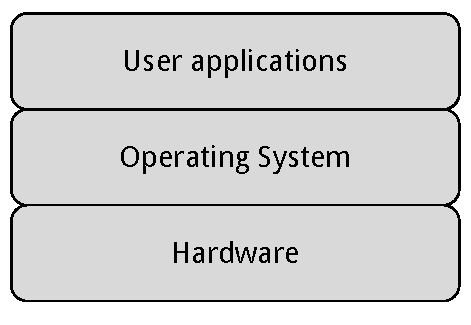
\includegraphics[scale = 1.0]{3-layers-stack.pdf}
\caption{A standard 3-layers-stack computer system}
\label{fig:3ls}
\end{figure}

This (relatively) simple architecture has proven to be very effective in delivering the IT services required
by companies, individual users and other organizations.

\vspace{0.5cm}

Neverthless, more complex computer systems organizations have been devised and used, in order to overcome some limitations
of the standard computer system model.

These computing environments are are known as \emph{Virtual Machines} (VMs) systems.
By itself, the term \emph{Virtual Machine} can have several meanings, so when using it is important to point out what we are
addressing. In section \ref{sec:vmclass} we will provide a classification of these meanings.
In general \emph{virtualization} provides a way of increasing the \emph{flexibility} of real hardware/software resources. When a 
physical resource is virtualized, it can appear to be a resource of a different kind or even a \emph{set} of different
resources (the same kind or different kind).

As an example, a single IA32 processor can be virtualized in a way that emulates more PowerPC processors. Once this is done, you
can build many standard 3-layer computer systems on top of each emulated PowerPC (virtual) processor, using unmodified OS and 
applications designed to be used on the PowerPC architecture.

\vspace{0.5cm}

We talk about Virtual Machines when we virtualize a physical computing enviroment (e.g a server machine) and get one or more 
independent virtual computing environment (the VMs), potentially different by the original one.

In the VMs terminology, each VM is also called \emph{guest}, whereas the virtualized physical computing environment is known as
\emph{host}.
The piece of software that provides the support for virtualization is called \emph{Virtual Machine Monitor} (VMM) or \emph{Hypervisor}.

You can virtualize nearly all the resources you wants: disks, network devices, memories or other peripherals.

\vspace{0.5cm}

Generally speaking VMs allow to build computer systems with more abstraction levels than the standard model has. This has important
advantages:
\begin{itemize}
  \item In terms of \emph{flexibility}, using VMs you can easily run programs compiled for a given Instruction Set Architecture (ISA) 
	and a given Operating System (OS) on top of a computer system that has a different ISA and/or a different OS. Using a standard
	system you would be bound to the ISA of your processor and the operating system installed on your machine. This flexibility can be 
	exploited in several situations, such as testing new software on different architectures (without physically have the
	machines supporting each different architecture), or run legacy applications on newer, more power-efficient hardware.

  \item In terms of \emph{protection}, VMs can provide multiple isolated execution environments running on the same phisical machine.
	This allows to execute different applications in different VMs (each VM can have its own OS), so that if an application has a
	security hole, an attacker cannot use the hole to do malicious attacks to an applications running on a different VM. 
	This scenary is still possible when applications are run in the same OS.
	
  \item In terms of resources usage, VMs can help to reduce hardware costs and power consumption, since they naturally improve 
	resource utiliziation. For instance, you can use only one physical server machine to provide multiple services (without 
	sacrifying isolation), using the 100\% of the machine resource, instead of using many underutilized server machines
	\footnote{Assuming, as often happens, that one or a few services don't utilize all the computing resource offered by
	a modern server machine.}. This results in money and energy saving.
	
  \item In terms of \emph{mobility}, you can easily migrate VMs (and so replicate them) to other locations, simply transmitting 
	some files through the Internet. This can also help avoiding setup times (software installation and configuration), 
	since through a VM you can convey a ready-to-use copy of a computing environment to the user.
\end{itemize}

The previous list is not exhaustive, but gives an idea of the services that virtualization can deliver, and makes clear the reasons
why IT departments make massive use of virtualization technologies.



\section{Virtual Machines classification}
\label{sec:vmclass}

As noted previously, the term \emph{Virtual Machine} can have several meanings. Therefore it is useful to give
a classification of the possible meanings (see \cite{ref:vmclassification} section 1.5 in \cite{ref:vmbook}).

First of all, VM can be divided in two categories:
\begin{itemize}
    \item \emph{System Virtual Machines}: these VMs provides virtualization at ISA level. This means that the VM is capable of executing 
	  arbitrary code compiled for a specified ISA.  System virtual machines provides a complete executing environment where
	  multiple processes can be run.
	  A system VM can then be used to run an OS that supports several applications, namely a standard 3-layers computer
	  environment.
	  
    \item \emph{Process Virtual Machines}: these VMs virtualize at the Application Binary Interface (ABI) level, providing
	  an execution environment for a single application. Since
	  applications are usually written in high level languages and so use an high level interface\footnote{For instance an OS 
	  system call interface, or the interface provided by an interpreted programming language.}, if we want to execute a single
	  application, the VM is only required to emulate the high level interface and/or a subset of the ISA\footnote{Typically 
	  unprevileged instructions, and instructions that are not problematic with respect to CPU virtualization (see \cite{ref:x86-virt}
	  and section 8.2 in \cite{ref:vmbook}).}. User applications are therefore provided with a virtual ABI anvironment.
\end{itemize}

\subsection{System level Virtual Machines}
System virtual machines can be further divided depending on whether the code executed in the VM (the guest) is of the same ISA
of the physical machine supporting the VM (host).

The same-ISA case is very common, since users are often interested in server consolidation (resource usage optimization), protection or
live migration, but don't care about executing code compiled for a specific ISA. Same-ISA VM are generally easier to design and 
are generally more suitable to be executed efficiently (e.g. the efficient hardware-based virtualization can be used in this case).

Same-ISA system VM can be further divided, depending on how the VMM is implemented:
\begin{itemize}
    \item Type 1 VMM (\emph{Native} VMM). In this case the VMM is a software component that runs on the physical machine (the host) 
	  without any OS support.
	  It's up to the VMM to interface directly with the physical resources of the server machines, such as
	  CPUs, memory and peripherals. Type 1 VMM can deliver a very good performance, but are more complex to design and require
	  more development efforts, since there is no OS providing basic services, abstractions, device drivers and the like.
	  An example of system including a Type 1 VMM is illustrated in figure \ref{fig:t1vmm}.
	  
    \item Type 2 VMM (\emph{Hosted} VMM). In this case the VMM it's just a regular OS process, that runs on the host OS along with other
	  processes. The VMM can access the physical resources of the host machine through the OS services. The OS support speeds up
	  the development process and make the VMM portable. On the other hand, performances are generally inferior with respect to the
	  Type 1 VMM. An example of system including a Type 2 VMM is illustrated in figure \ref{fig:t2vmm}.
\end{itemize}

\begin{figure}[bt]
\centering
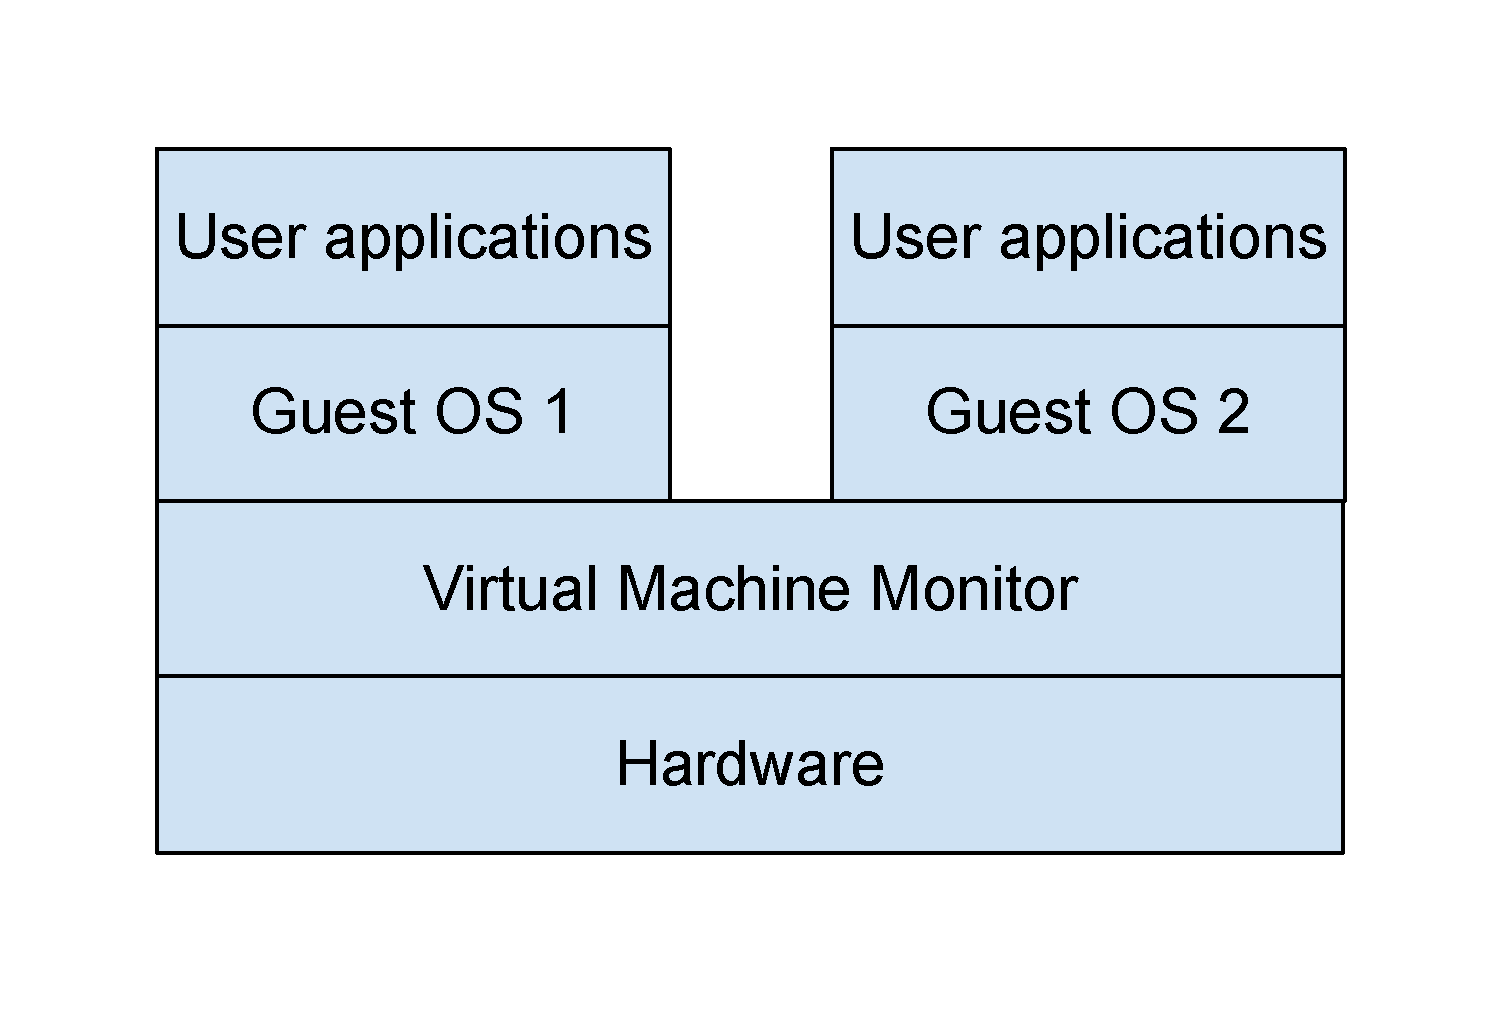
\includegraphics[scale = 1.0]{type-1-vmm.pdf}
\caption{An example of system using Type 1 VMMs.}
\label{fig:t1vmm}
\end{figure}

\begin{figure}[bt]
\centering
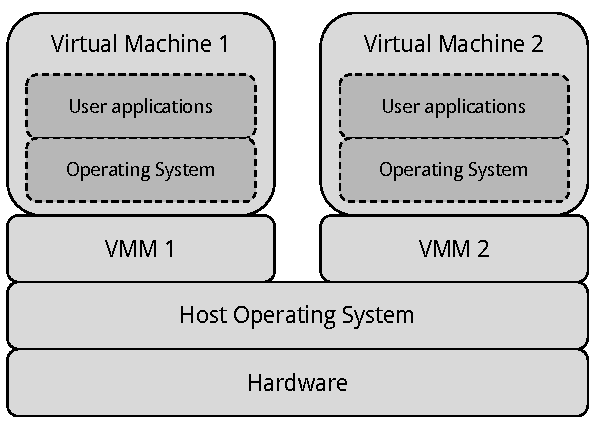
\includegraphics[scale = 1.0]{type-2-vmm.pdf}
\caption{An example of system using Type 1 VMMs.}
\label{fig:t2vmm}
\end{figure}



\vspace{0.5cm}

The different-ISA case is useful if you want to run legacy software on modern machines\footnote{Game console emulators are a common case 
of this kind of VM.} or if you want to test your software for compatibility with other architectures. In this case a VMM is basically a
full system emulator, capable to emulate the complete behaviour af a complex computer system.


\subsection{Process level Virtual Machines}
A very similar secondary classification applies also to process virtual machines, although at the ABI level. A VM can expose to the
application it executes (the guest application) the same ABI exposed to a regular process excecuting in the host system, or expose a 
completely different ABI.

Here the common case is when the ABI is different. The Java Virtual Machine is an example of this VM type: it executes code written 
conforming to an ABI (the Java bytecode) which is different by the ABI offered by the host OS. In this case the JVM engine is the VMM.
All interpreted language engines are VMs of this kind. Process VMs are also used for other purposes, such as runtime optimization
of binary code (see chapter 4 of \cite{ref:vmbook}), or binary translation in general.

\vspace{0.5cm}

The same-ABI case is just the concept of multiprogrammed OS, namely an OS capable of virtualize the CPU and
memory, offering to each process a \emph{virtual processor} and a \emph{virtual memory}. These two virtual resources make up
the enviroment (which provides some limited degree of isolation) where an OS process lives. We are so used to the multiprogramming
concept that we don't even think of it as being a form of virtualization. In this case the VMM is the OS itself (together with
the ISA which is designed to efficiently support multiprogramming).


\section{Virtual Machine Implementation}
\label{sec:vmimpl}

As showed in section \ref{sec:vmclass}, there are many types of conceptually different virtual machines.
Neverthless, all the VMs deal with executing code written for a certain environment (source code, or guest code),
using another environment (the host environment). This is a form \emph{emulation}: the term emulation refers to \emph{the process of
implementing the interface and functionality of a system on a system having a different interface and functionality}
(\cite{ref:vmbook} page 27).

The basic techniques employed to implement emulation are three: interpretation, dynamic translation, and hardware-based virtualization.
These techniques can be used alone or in combination to provide the virtual environment we want to implement.
Nowadays VMMs generally use a combination of the three methods.


\subsection{Interpretation}
The naive emulation technique is known as \emph{interpretation}.
Basically, the VMM has to do in software what a physical CPU would have done
in hardware. Take the current instruction (or statement, if we are dealing with high level languages VMs), excecute it updating the
VM status (which is an in-memory representation of all the VM resources, like registers, memories and the like), and go to the next
instruction. The VMM would then be implemented as a loop that, in each iteration, performs the fetch, decode and execute phases of
instruction execution.

\vspace{0.5cm}

Although writing an interpreter for a modern ISA or an interpreted programming languages can be a very long and complex process,
because of the complexity of the source language, the technique is conceptually easy. You just have to read an Instruction Set 
specification or a Programming Language specification and implement all the possible instructions/statement strictly respecting
the specified behaviour.

Being simple, this method is generally terribly inefficient if compared to the native execution of the source code on a processor
designed to execute the source ISA, because for each source instruction the VMM has to execute many host instructions (e.g. 30-100)
to perform in software all the necessary operations. In other words, the average \emph{translation ratio} is very high (e.g. 40).
On the other end, a big advantage is that the VMM has always the control over the execution of the source program, because it is 
executing the program step by step.

Many tricks can be implemented in order to improve the emulation performances. Some of these tecniques can be found in \cite{ref:vmbook}
(sections 2.1 through 2.4).


\subsection{Dynamic Translation}
A more sophisiticated form of emulation is called \emph{dynamic translation} or \emph{binary translation} or 
\emph{Just In Time compliation}, depending on the context.

Having to translate a source code in something else, an idea is to translate it into equivalent binary code that can be directly
executed on the host CPU. The VMM does this translation \emph{on the fly}, as soon as the source code is fetched from memory.
The method is intended to amortize the costs of interpretation, doing the repetitive work (fetch and decode) once or a few
times. 
The code execution step of a source instruction or a block of instructions, namely the translation, is generated once (or a few times)
and saved in a \emph{Code Cache}. The next time the source program flow goes through that block of source instructions, we don't have
to fetch, decode or translate, but just to execute the translation block.
The blocks of translated instructions can be connected directly to each other using native jump instructions, 
in the way suggested by the source program flow. After some time the code cache will become the complete translation of the source program
into the host ISA.

The final result is that the average translation ratio can be very close to 1 (e.g. less than 4), giving a nearly native performance,
or at least a performance that is acceptable also for performance sensitive applications.

\vspace{0.5cm}

The whole process is of course way more complicated than what has been presented here. Several problems are present, such as the 
\emph{code-discovery} problem that makes impossible to do a static translation, or the \emph{code-location} problems, that is due
to the different address space of the guest and host systems, or the state mapping problem, that is the way the VMM maps guest registers
and similar resources to the host ones.

Similarly to the interpretation method, with dynamic translation the VMM has (or can easily get) complete control over the guest code
execution: While doing the translation, it can put \emph{traps}\footnote{Point in the code that interrupts the guest
execution and give control to the VMM directly, or indirectly thorugh the host OS.} in the guest code wherever it wants.

For further informations on dynamic translation, see \cite{ref:vmbook} (sections 2.5 through 2.9).


\subsubsection{The same-ISA case}
\label{sec:sidt}
Interesting enough, interpretation and dynamic translation can make sense also in the same-ISA case. In this case the translation is
simplified, and most of the time the source code can execute natively on the host machine, without performance losses.

However there are some instructions that cannot be executed natively, because they access physical resources, because
are trying to access resources that do not exists on the physical machines, or because they are not easily virtualizable (see
\cite{ref:x86-virt} and section 8.2 of \cite{ref:vmbook}).

\vspace{0.5cm}

As a typical example, memory accesses addressing the I/O space or the memory mapped I/O can have side effects and then must be emulated 
in software. If the instruction was intended to access a physical resource that exists on the host, like a network adapter, the VMM 
cannot allow direct access to the device, because other processes or the host OS could be accessing the same device at the same time,
and certainly the host network driver and the guest network driver are not aware of each other.
If the instruction was intended to access a virtual network adapter (that doesn't exist on the host), the I/O instruction must be trapped
in order to emulate the device behaviour in software.


\subsection{Hardware-based virtualization}
\label{sec:hbv}
Due to the widespread use of VMs, the processor vendors have introduced processor extensions that allow for efficient and safe execution
of guest code in the same-ISA case. These hardware assists are intended to overcome some of the common problems arising when using
dynamic translation techniques, and at the same time they make it easy to execute guest code natively.
For the x86 ISA, both AMD and Intel have proposed their extensions, AMD-v (\cite{ref:amd-v}) and Intel VT-x (\cite{ref:intel-VT-x}).
These features provide all the means necessary to fully virtualize the x86 ISA. Since they fairly complex, we will only outline those
aspects that are intersting with respect to our work.

\vspace{0.5cm}

When the extension are present, the CPU is able to switch to a special mode, that we will call \emph{VM mode}, through a so called
\emph{VMEnter} instruction and switch back to normal mode through a so called \emph{VMExit} instruction.
When in VM mode, the CPU can execute guest code in a controlled environment. When necessary, the CPU can switch back to normal mode, 
starting to execute host code (VMM, OS or other processes).
The switch operation between the the host world and the guest world is conceptually similar to the more familiar process context switch,
since it includes saving the host (guest) state and loading the guest (host) state. These operation are done in hardware but are
still very expensive, expecially if we consider the additional software overhead involved in this host-guest transition, due to
OS operations and possible userspace/kernelspace transitions that could be necessary to transfer the control to the VMM or to the
guest.

The VM switches are necessary in some situations, such as dealing with I/O operations (see \ref{sec:sidt}), or when we want
to deliver an interrupt to the guest.

Since VM switches are very expensive, but sometimes necessary, trying to minimize them is fundamental if a VMM
wants to deliver good I/O performance.

\chapter{Working environment}
In section \ref{sec:vmclass} we introduced a classification of Virtual Machine systems.

The work presented in this thesis is restricted to same-ISA System Virtual Machines, where the Virtual Machine Monitor is a type 2 VMM.
In other words, we will deal with VMs that able to run an arbitrary OS compiled for the host ISA. The guest OS can in turn provide an 
execution environment for many user application.
Since the VMM is of type 2, it is implemented as a regular process in the host OS, and can make use of all the OS services.
We can therefore access the physical resource without requiring administrator previleges.

We also restrict our work to VMMs that make use of hardware-based virtualization, because the optimizations we will intrduce are
particularly effective in limiting the amount of VM switches between the host world and the guest world. Since these VM switches
are very expensive with hardware virtualization, the performance gain is significant.

While the assumptions made may appear restrictive, they are not at all. The class of VMMs that we consider is extremely 
common in the world of computing. They are used in datacenters and IT departments for server consolidation, 
application isolation, or to provide users/developers with zero-setup computing environments and other application in which it's
not important that the computing environment supported the VM has a different ISA from the host ISA.

\vspace{0.5cm}

Several VMM software belonging to the considered class are available. QEMU, VirtualBox, VMWare, Parallels, Windows
Hyper-V or Windows VirtualPC are among the most common examples of this kind of VMMs. These software tools are extremely widespread
and for this reason performance optimizations in these area are certainly useful.

This said, we have chosen the QEMU-KVM Virtual Machine Monitor for implementations and tests, although our optimizations are
relevant to the entire class of VMMs.

A GNU/Linux-based operating system (Archlinux) have been used on the host machine. The guest OS is generally Archlinux, but 
some tests have been performed with FreeBSD as a guest, too. Although Linux is a kernel and not a complete OS, in the following we 
will use  the expression ``Linux OS'' to actually mean ``GUN/Linux-based OS'', for the sake of simplicity.

\vspace{0.5cm}

Since our optimizations concern network performance, we had to choose a network device to work with. The \emph{e1000} class of 
network devices was chosen, since it is emulated by the vast majority of VMMs and supported by the main OSs (Windows, Linux, FreeBSD).


\section{QEMU features}
QEMU is a free, open source and multi-platform type 2 VMM, that makes use of dynamic translation to achieve good emulation performance.
QEMU-KVM is a QEMU branch that extends the original software to take advantage of hardware-based virtualization.
Whenever possible, QEMU-KVM uses hardware virtualization in order to execute guest code natively.
In the following we will use the terms QEMU and QEMU-KVM in an interchangeable manner.
At the date of this writing, the QEMU-KVM version number is 1.2.0, so we will refer to that version.

QEMU is a very flexible tool:
\begin{itemize}
    \item It supports process virtual machines: by means of dynamic translation it can execute on the host OS a single program compiled 
	  for an other ISA. This operating mode is called \emph{User mode emulation}.
	  
    \item It supports system virtual machines: by means of dynamic translation and hardware-assisted virtualization (when possible) it
	  can emulate full computer systems (including common peripherals), supporting unmodified operating systems. This operating
	  mode (which is the one we are interested in) is called \emph{Full system emulation}.
	  
    \item It supports various architectures, including  IA-32 (x86), x86-64, MIPS R4000, Sun's SPARC sun4m, Sun's SPARC sun4u,
	  ARM development boards (Integrator/CP and Versatile/PB), SH4 SHIX board, PowerPC,
	  ETRAX CRIS and MicroBlaze architectures.
	  
    \item It can emulate Symmetric Multiprocessing Systems (SMP), making use of all the CPUs that are present on the 
	  host system.
	  
    \item It is able to emulate various peripherals, such as hard disks, CD-ROM drives, network cards, audio interfaces, 
	  or USB devices.
	  
    \item Like similar hypervisors, it is able to provide its VM with network connectivity. The way this can be done will be
	  presented in section \ref{sec:qemunet}.
	  
    \item It does not normally require administrative rights to run. In our experiments administrative rights won't be
	  necessary.
\end{itemize}

QEMU is able to emulate the \emph{e1000} class of PCI network devices\footnote{To be more precise, the emulated hardware exposes
to the guest OS the PCI device ID of the 82540EM model.}, as well as other network devices (RTL8139C+, i8255x (PRO100), 
NE2000 (RTL8029), AMD PCNET II (Am79C7070a)).

In addition to that, QEMU support the \emph{Virtio} framework, that exposes a paravirtualized network device, virtio-net, intended 
to be used for high performance networking. The Virtio paravirtualized soution will be analized later.



\section{QEMU internal architecture}
In this section we will illustrate those details of QEMU implementation that are necessary to understand in order to reach our
goals.

\subsection{QEMU event-loop}
QEMU is an event-loop based software, and is implemented as a single-process multi-threaded application. 
One thread, referred to as \emph{IOThread}, executes the event-loop, waiting for new events to happen\footnote{This is 
implemented in \texttt{main-loop.c}}.
The waiting routine is a \texttt{select()} system call, which is not the most efficient choice on Unix-like systems
\footnote{ \texttt{poll()}, and espcially Linux \texttt{epoll()} or BSD \texttt{kqueue()} are more efficient},
but is more portable across different platforms.

\vspace{0.5cm}

The file descriptors associated with the \texttt{select()} can be associated to regular files, sockets, device files (such as TAP 
devices), or even special in-kernel objects, such as POSIX timers, signals and eventfds. These file descriptors are used by QEMU to let
the VM communicate with the host, and possibly with the rest of the Internet. In other words, they are used for performing the I/O 
operations requested by the VM. Of course the guest OS still performs I/O operations accessing I/O ports or memory-mapped I/O (MMIO) in 
his physical address space and is unaware of being emulated.

\vspace{0.5cm}

The QEMU core codebase offers to the QEMU developer an API that can be used to implement emulation of the devices.
The API also provides two useful abstractions: the QEMUTimer and the QEMUBH. 

QEMUTimers are a one-shot absolute timers, that can be 
used to execute a callback function at a certain point of time in the future. The callback is always executed by the IOThread, when it
recognizes that the deadline has been passed. The QEMUTimers are supported
by the Linux OS with a single one-shot relative POSIX timer\footnote{Similar mechanisms are used in other OS, or if POSIX timers are not
available under the Linux OS}, which is always (re)armed to expire - waking up the event-loop - at
the earliest deadline. The expire check for QEMUTimers is done at the end of each event-loop iteration, even if the event-loop was 
waken up for a reason different from the POSIX timer expiration. In the current implementation, moreover, every time the POSIX timer
is rearmed, the relative deadline is forced to be greater or equal that 250 $\mu$s\footnote{For more information about the QEMUTimer
interface and implementation, please refer to the file \texttt{qemu-timer.c} in the QEMU project root directory.}.

\vspace{0.5cm}

QEMUBH is the QEMU abstraction of the \emph{bottom half} concept, widely used in OS driver implementation. A QEMUBH can be seen as
a QEMUTimer that expires as soon as possible. In practice when a QEMUBH is scheduled, it notifies the event-loop, which in turn 
wakes up (or finishes the current iteration and begins another iteration) and execute all the callbacks of currently scheduled QEMUBHs.
Therefore the QEMUBH callbacks are always executed by the IOThread, similarly to the QEMUTimer callbacks\footnote{For more information
about the QEMUBH interface and implementation, please refer to the files \texttt{qemu-aio.h} and \texttt{async.c} in the QEMU project
root directory}. This feature is very important in terms of parallelism, as will be clear in the following chapters.

\subsection{VCPU Threads}
The IOThread, while executing the event-loop, handles all the interactions between the VM and the external world.
The guest code, however, is executed by one or more threads, that we will call \emph{VCPU threads}. In the current implementation QEMU
creates as many VCPU threads as the number of SMP processors specified by the users.
When using hardware-based virtualization (we made this assumption at the beginning of this chapter), a VCPU thread continuously
switch between the VM mode and the normal mode (see section \ref{sec:hbv}).

When the VCPU tries to execute an I/O operation - accessing I/O ports or MMIO - a VMExit happens. There could be other events
that cause a VMExit, but I/O operations are the type of events we are interested in. On a VMExit the VCPU stops executing guest
code and starts executing QEMU code, in order to handle - if is the case - the event that caused the VMExit.
When the event is handled, the VPCU executes e VMEnter and continues to run the guest code.

\vspace{0.5cm}

Since multiple threads are involved, and all of them - IOThread included - can access the shared structures used by the emulator
(e.g. the structures employed to implement the virtual devices), mutual exclusion is required. In the current implementation the
mutual exclusion is guaranteed by a single big-lock, called the \texttt{iothread lock}.

Therefore, on every VMExit a VCPU has to acquire the \texttt{iothread lock} before it can handle the event. After the event has been
handled, the VPCU thread release the \texttt{iothread lock} and execute a VMEnter instruction.
Similarly, the IOthread has to acquire the \texttt{iothread lock} every time it wakes up for event handling, and release the lock
only when the event-loop iteration terminates.

Putting all together, the figure \ref{fig:qemuthreads} depicts the QEMU thread scheme.

\begin{figure}[bt]
\centering
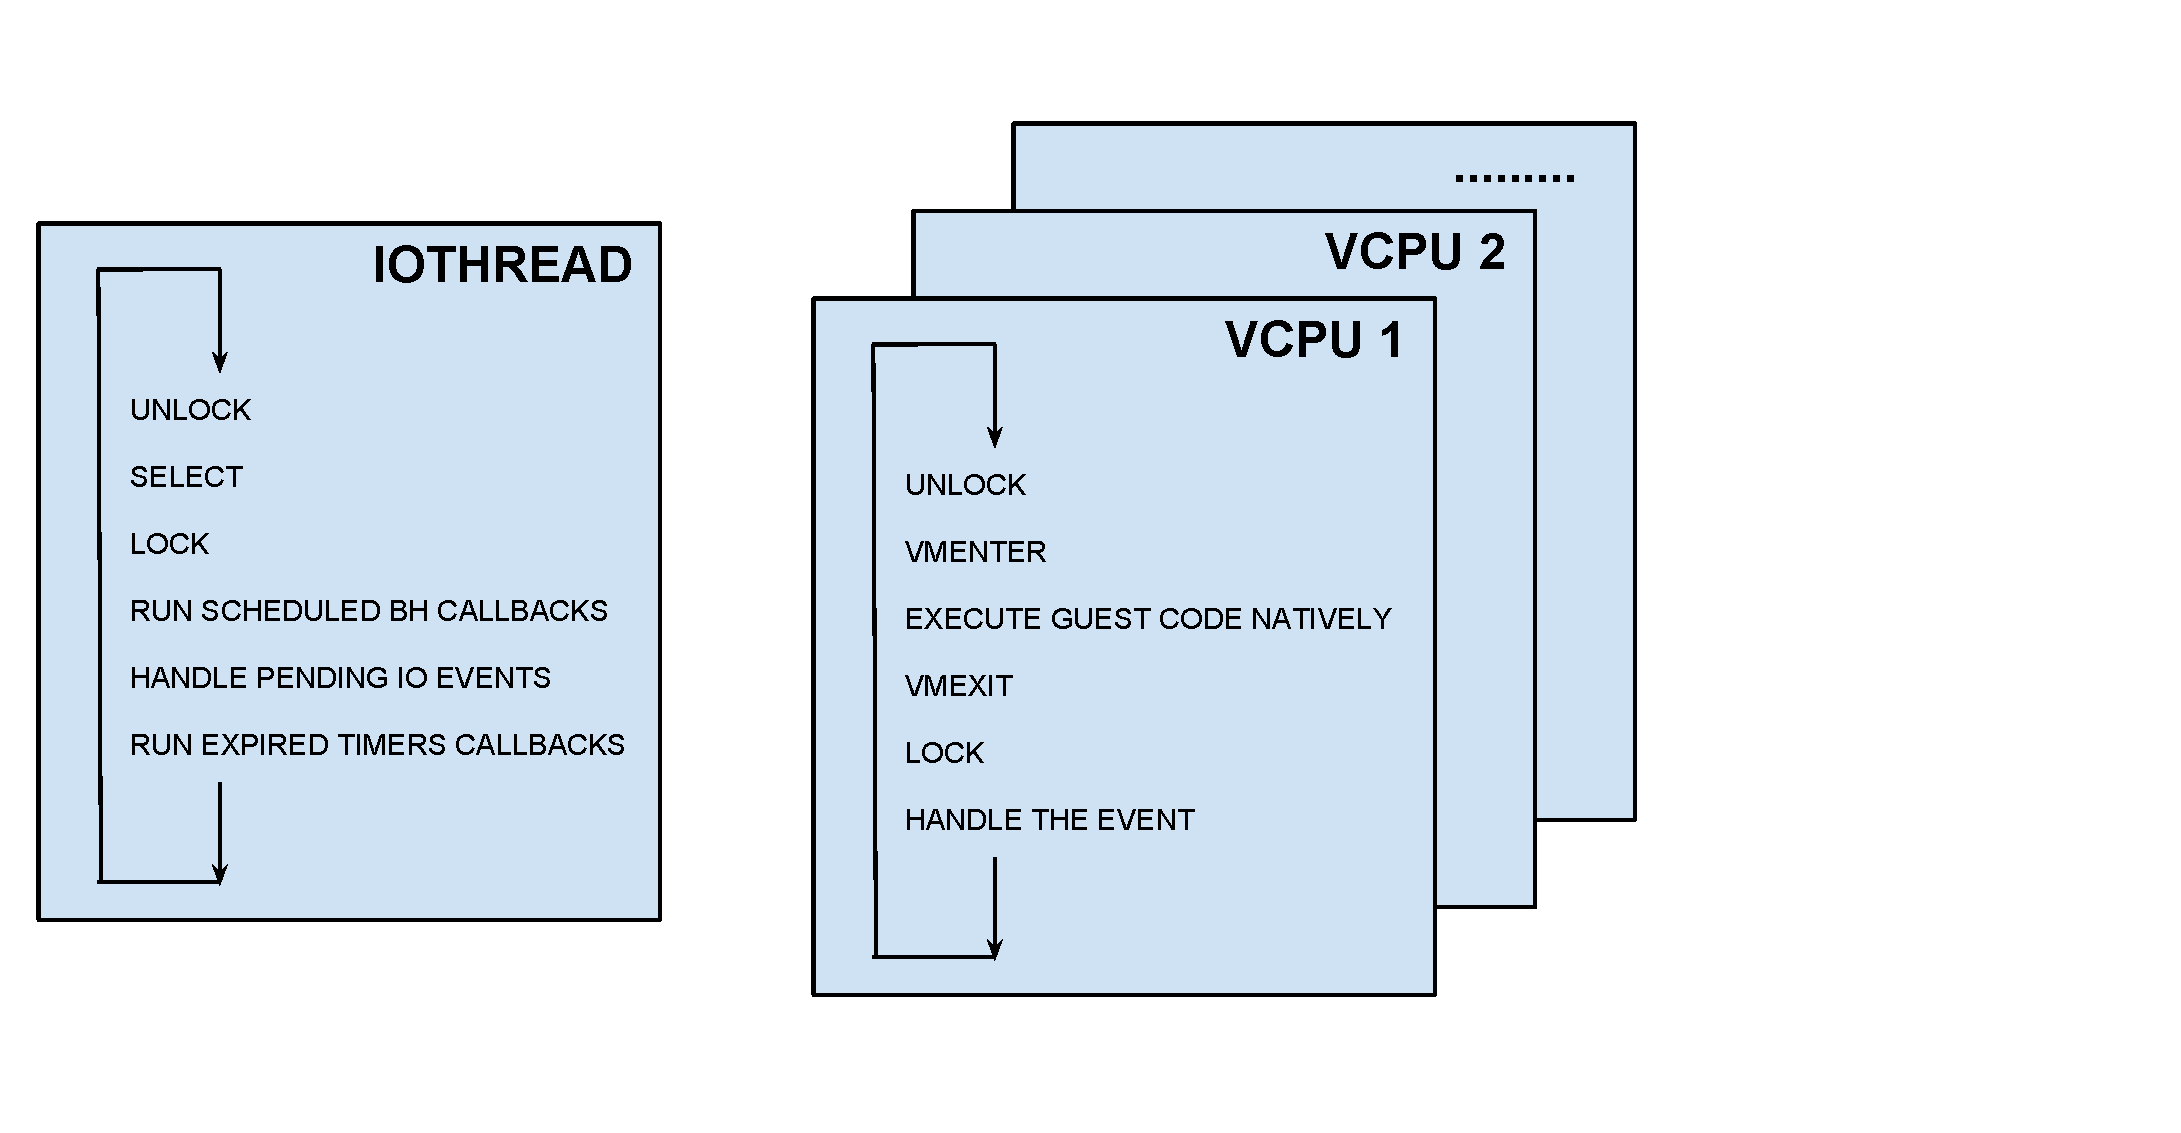
\includegraphics[scale = 0.45]{qemu-threads.pdf}
\caption{QEMU thread scheme.}
\label{fig:qemuthreads}
\end{figure}



\subsection{Networking architectures}
\label{sec:qemunet}
When running a VM it is of fundamental importance to make possible for the guest to communicate with the outside world using the
networking infrastructure, otherwise the VM itself would be an useless computing box.

Since the VM it's a software entity, however, it isn't connected to any real network. Therefore the hypervisor has to provide some
form of network infrastructure virtualization, so that the guest OS thinks its (virtual) network device is connected to a physical
network and can then exchange packets with the outside.

\vspace{0.5cm}

All the hypervisors cited previously (QEMU included) provide the VM administrator with a few virtual network infrastructure modes, 
so that she can choose the best way to connect her VM.

Three modes are commonly employed:
\begin{itemize}
    \item NAT mode. In this case the guest OS thinks to be physically connected to a completely fake LAN, entirely emulated inside the 
	  hypervisor. The VMM usually emulates a DHCP server, a DNS server and a gateway router, so that the guest OS can configure
	  its network interfaces and its routing tables
	  and communicate with the outside world. When the guest sends a TCP/UDP packet on the fake LAN, the VMM intercepts the packet,
	  performs address translation (NAT) turning the guest source IP (the guest IP) into the host IP and sends the packet towards
	  its destination using the host OS services (thus the host OS routing tables). The inverse translation is performed when
	  receiving a packet.
	  
	  In this way the VM is easily provided with Internet connectivity, but it's not visible form the outside
	  and cannot communicate with other VMs present on the same host.
	  In QEMU this mode is called \emph{Usermode networking}.

    \item Host-only mode. Also in this case the guest OS thinks to be physically connected to a LAN. The LAN is emulated
	  by means of a software bridge (that emulates a layer-2 network switch), and the VM is connected to a port of the bridge.
	  More VMs can be connected to the same bridge, making inter-VM communication possible. The software bridge can be internally
	  implemented in the hypervisor, or can be an external software bridge.
	  
	  Whit QEMU this mode can be set up on a Linux host using the in-kernel bridging and TAP interfaces. Each VM is assigned a TAP
	  interface where can write/read ethernet frames, and all the TAPs are bridged together to the in-kernel bridge.
	  In this way a frame sent by the guest is written by QEMU to its associated TAP and is therefore routed by the bridge
	  to the correct destination TAP. The receiving QEMU process can then read the frame from the TAP and push it to its VM.
	  In this case no DHCP or DNS server is emulated, and you have to configure yourself the network of each VM\footnote{The 
	  configuration can be static or you can run a DHCP server on one of the VMs connected to the bridge.}.
	  Since the software bridge itself has its separate network interface, also the host can communicate on the LAN.
	  
    \item Bridged mode. This mode is an extension of the host-only mode. The only difference is that a physical host network interface
	  is also bridged to the VMs LAN. Since the physical interface becomes a bridge port, the host can access the physical network
	  through the software bridge interface.
	  In this way the host can share its connectivity with all the VM connected to the software bridge. If the physical interface
	  is connected to a LAN, with this configuration the VMs LAN appears to be part of the physical LAN.
	  
\end{itemize}
	
Clearly the NAT mode is not interesting with respect to our goals, since it is only intended to be a way the VM can easily obtain
Internet connectivity, and it's not intended to be a flexible networking mode. Instead we will consider host-only mode, since we
are intersted in optimizing the communication performance between two VMs on the same software bridge or between a VM and the host
bridge interface. In this work it would make no sense considering to bridge also the host physical interfaces (bridged mode), 
because we optimizing performance of physical network adapter it's not among our goals.


\subsection{Network frontend and backend}
\label{sec:frontback}
In order to implement a specific networking architecture, the QEMU implementation includes a degree o separation, namely an interface,
between the piece of code that emulates the network device and the code that provides access to the chosen networking model.
This is done because the two subsystems are completely independent, and you can easily combine every virtual network device with
every networking access mode.

Using the QEMU terminology, the network device emulation is also called \emph{network frontend}, and the networking access mode is
called \emph{network backend}. 

\vspace{0.5cm}

In our case the network frontend is ``e1000'' and it's implemented within the file hw/e1000.c (in the QEMU project root directory).
This source file is the only one that contains code which is specific to the e1000 class of networking devices, exporting to the rest 
of the system the same interface exported by the other network devices.

The network backend can be
\begin{itemize}
    \item ``user'', which implements Usermode networking.
    \item ``tap'', which is an implementation of host-only/bridged networking that relies on TAP devices and in-kernel bridges.
    \item other implementations of host-only/bridged networking that use a different software bridge solutions, maybe in conjunction
	  with TAPs and in-kernel bridges. The ``VALE'' backend (\cite{ref:vale}) is an example of high performance alternative 
	  implementation of the host-only/bridged networking access mode.
\end{itemize}

\vspace{0.5cm}

Frontend and backend can be seen as two peers connected to each other that are able to exchange ethernet frames. Each peer exports a 
\texttt{receive} method that accepts an ethernet frame as argument\footnote{The ethernet frame frame can be specified with an address 
and a length, or with a scatter-gather array.}. That method will be invoked whenever the other peer wants to send a frame.

In this way, when a frontend wants to send a frame to the network, it invokes the \texttt{qemu\_send\_packet} function provided by the QEMU
networking API, that will invoke the \texttt{receive} method exported by the backend. The backend \texttt{receive} method will push the
frame onto the network, in a way that is specific to the backend itself.

On the other direction, when the backend gets a frame from the network, it invokes the \texttt{qemu\_send\_packet} function, that will in turn
invoke the \texttt{receive} method exported by the frontend. This method will push the frame into the guest system in a way that is
specific to the network device model.

The frontend-backend communication is depicted in figure \ref{fig:frontback}.

\begin{figure}[bt]
\centering
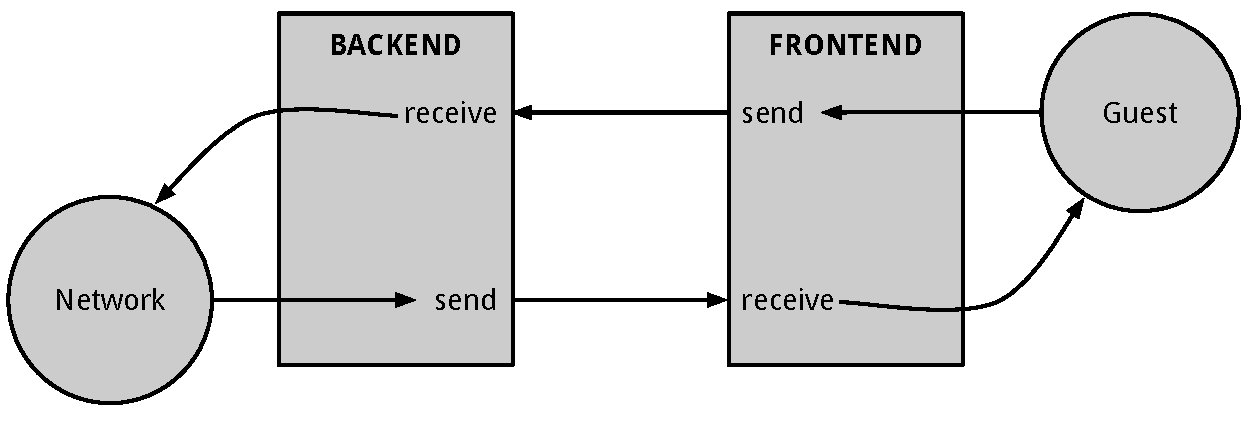
\includegraphics[scale = 0.60]{frontend-backend.pdf}
\caption{Interface between network frontend and network backend.}
\label{fig:frontback}
\end{figure}



\section{The e1000 class of network adapters}
In this section we will illustrate some features and some details about the inner working of an e1000 ethernet network adapter.
Once again, we will only describe those aspects that are relevant to our goals.
The complete specification can be found in %cite Intel.

\vspace{0.5cm}

Since the network communication is extremely important in the IT world, the market constantly pushes hardware vendors to produce high
performance, low-power, fully featured flexible network devices.

As a result, modern network devices are very complex. To get an idea of this complexity, one can observe that a device can implement 
more then a hundred of software-visible registers. The complexity is the price to pay in order to get high flexibity and several useful
features. Flexibility helps the IT administrator to tune the device parameters in order to find the right tradeoff between performance and 
power consumption, throughput and latency, and the like.
The rich set of features the device come with helps to adapt the device to different usage patterns and allows for performance 
optimizations (expecially for TCP/IP traffic) when offloading capabilities are present.

Hardware offloading features are supported by virtually every recent network adapter.
The most common feature are
\begin{itemize}
    \item Checksumming offload. When this feature is present, the device computes in hardware the checksums required by the main Internet 
	  protocols, such as IP, TCP and UDP. This saves the OS to do this work in software, which could be very expensive, expecially 
	  with checksums that are computed also on the payload and not only on the protocol header (e.g. TCP and UDP checksums).
	  
    \item TCP Segmentation Offload. When this feature is present, the device is able to do the TCP segmentation in hardware, splitting
	  a TCP segment over multiple ethernet frames. The segmentation is necessary because the real MTU of a TCP connection is almost
	  never greater than 1500 bytes (the ethernet original MTU), but the TCP window is commonly greater than that value. The OS
	  is then forced to do the splitting. With the feature present, however, the OS can send to the device driver a frame containing a 
	  TCP segment which is greater than the MTU\footnote{Up to 64KB with the Linux kernel.}. The device driver can pass the packet to
	  the device that perform the segmentation in hardware and send multiple ethernet frames.
	  Apart from the obvious speed-up obtained because the operation is done in hardware rather then in software, this mechanisms has 
	  an important positive side effect. The network overhead necessary to traverse the TCP/IP stack is suffered only once, for a
	  big TCP packet, instead of once for each MTU-sized fragment. This clearly amortize the kernel per-packet overhead.
	  
    \item Scatter-gather capability. When this feature is present, the device is able to send a frame that is stored in multiple non
	  contiguous fragments in the machine physical memory. Therefore the OS is not forced to linearize (gather) the fragments,
	  avoiding the copy overhead. This is useful specially when the OS wants to send large packets. In other words the device is 
	  gather-capable.
\end{itemize}
The e1000 devices have this three features.


\subsection{Data interface with the driver}
Being high performance devices, modern network adapters rely on Direct Memory Access (DMA) operations and interrupts.

When the device driver wants to send an ethernet frame through the adapter, it has to tell the device where the frame is stored
in physical memory and how long it is\footnote{When dealing with fragmented frames, the driver has to specify somehow a scatter-gather
array.}. Once the device knows where the frame is, it can directly access the physical memory\footnote{In this example we assume
there isn't any IOMMU.} and send it on the wire. More commonly, the frame is DMA'ed into an internal buffer for further processing before
being sent on the wire, but this is just a detail.

When the adapter receives a frame from the wire, it has to store it in the machine physical memory. For this reason, the device driver
has to tell the adapter where it can store incoming frames, before the frames actually came. If the adapter doesn't know how to put
incoming frames, it cannot accept them.

\vspace{0.5cm}

It is clear that there must be a well-defined interface between the driver and the device. This interface is known as \emph{ring}.
A ring is a circular array of \emph{descriptors} that are used to exchange address/length information\footnote{Being an array a ring is a 
contiguous zone in the physical memory.}. A network adapter have at least two rings.
The first one is the \emph{TX ring} and it is used with outgoing frames, whereas the second is the \emph{RX ring}, and it is used with
incoming frames. Network adapter can have multiple TX/RX rings with possibly different policies and priorities, so that one can
do some traffic engineering.

However, the e1000 adapter model emulated by QEMU has one TX ring and one RX ring. The array length, namely the number of descriptors,
can be decided by the driver to a certain extent. In e1000 it must be a power of two and not more than 4096.


\subsubsection{TX ring}
\label{sec:txring}
The e1000 TX ring is an array of $N$ TX descriptors. Each TX descriptor is 16 bytes long and contains the address (in physical memory) and the
length of a frame (or a frame fragment) that is going to be sent or that has already been sent. The descriptor contains also flags that
can be used to specify options, and status bits. 

Two index registers are implemented for the synchronization between the driver and the adapter:
The TDT register (Transmit Descriptor Tail) and the TDH register (Transmit Descriptor Head). These are \emph{index} registers since
their value are array indexes with respect to the TX ring descriptors array.

At the start-up, TDT and TDH are initialized by the driver to the same value, usually 0. When the driver wants to send a new frame,
it writes the physical address and the length of the frame in the TX descriptor pointed by the TDT register and then increments the TDT
register itself. Since the descriptor array is circular, the TDT must be set adequately.

When the adapter recognizes that TDH is different by TDT, is knows that there are new frames to transmit, and start processing the
descriptor pointed by TDH, sending on the wire the frame pointed by the descriptor (if is the case), and then increments the TDH register.
The adapter stops the processing only when TDH has the same content as TDT has. A write access to the TDT register is therefore the
way the device driver notifies the adapter that there are new frames ready to be sent.

When the driver increments the TDT, the descriptor previously pointed (the one that has just been written) is committed to the hardware,
and the hardware owns it until the decriptor is processed.

Therefore, in each moment the ring is partitioned in two contiguous parts: The descriptor owned by the hardware, which are waiting
to be sent on the wire, and the descriptors owned by software, which are free to be used by the driver to commit new frames.

In order to prevent the index registers to wrap around, the driver should not never use a TX descriptor if this is the very last free
TX descriptor. This happens when TDT is shuch that incrementing it circularly would cause TDT == TDH. When the TX ring is in this
state (TX ring full), the driver should stop transmitting. The transmission can be enabled again when the hardware process some descriptors,
incrementing TDH.

The figure \ref{fig:txring} depicts the TX ring with its index registers.

\begin{figure}[bt]
\centering
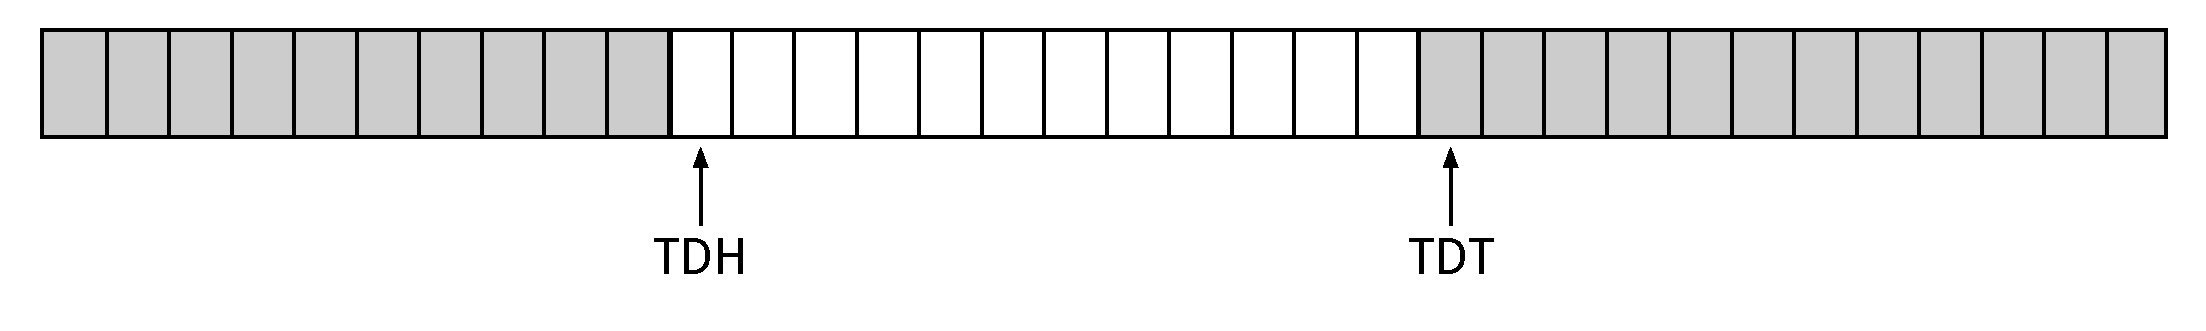
\includegraphics[scale = 0.35]{tx-ring.pdf}
\caption{The e1000 TX ring with its index registers. The grey area contains software-owned descriptors, while the white area
	contains hardware-owned descriptors.}
\label{fig:txring}
\end{figure}


\subsubsection{RX ring}
\label{sec:rxring}
The e1000 RX ring is an array of $N$ RX descriptors. Each RX descriptor is 16 bytes long and contains the address (in physical 
memory) and the length of a frame that has been received by the adapter, or only the address of a memory location that can be
used by the adapter to store an incoming frame. The descriptor contains also flags that can be used to specify options and status bits.
Two index registers are implemented for the synchronization between the driver and the adapter:
The RDT register (Receive Descriptor Tail) and the RDH register (Receive Descriptor Head). These are \emph{index} registers since
their value are array indexes with respect to the RX ring descriptors array.

At the start-up, the driver initializes RDH and RDT to 0. At this point, the adapter still doesn't know of any memory buffer where it
can store incoming frames, so it cannot receive anything.
To give the hardware memory buffers to work with, the driver puts the physical address of a memory buffer\footnote{How the memory 
buffer is allocated depends on the OS and on how the driver is implemented.} in the RX descriptor pointed by RDT and increments 
RDT circularly. Writing to the length field of the RX descriptor is useless, since this value is not used by the device. It's important to note
that the size of the memory buffer must be greater or equal then the maximum frame length, since we cannot know in advance how long
a future frame is going to be.

A write access to the RDT register is therefore the way the device driver notifies the adapter that there are new memory buffers ready
to be used to store incoming frames.

If the adapter sees that RDH is different by RDT, it recognizes to have memory buffers available, and starts accepting incoming frames.
When a new frame arrives from the wire, the adapter fetches the RX descriptor pointed by the RDH register, copies the frame to the address
contained in the RX descriptor, writes back the length of the received frame to the RX descriptor itself and increments the RDH register
circularly.
At this point, if programmed to do so, the device would normally sent an interrupt (see section \ref{sec:e1000int}, in order to tell
the driver there are new received frames ready to be pushed to the kernel network stack.

When the driver increments the RDT, the descriptor previously pointed (the one that has just been written) is committed to the hardware,
and the hardware owns it until the decriptor is used.

Therefore, in each moment the ring is partitioned in two contiguous parts: The descriptor owned by the hardware, which can be
used to store new incoming frames, and the descriptors owned by software, which are unused or point to received frames ready to
be pushed to the network stack.

Similarly to what happens the TX ring, in order to prevent the register indexes to wrap around, the driver should never increment the RDT
register if the increment would cause RDT == RDH. When this situation happens (full RX ring) the driver should stop giving memory buffers to
the adapter. When new frame are received, the hardware increments RDH, and so it is possible to restart.

The interrupt routine should then push the arrived frames to the kernel and provide the adapter with more memory buffers (incrementing
the RDT), otherwise the adapter cannot accept more incoming frames.

A common strategy is to try to keep the RX ring always full. In order to do this, at the startup
the driver writes $N-1$ RX descriptor with the address of $N-1$ memory buffers, and set RDT to $N-1$, so that the ring is full.
Every time an interrupt arrives, the interrupt routine pushes the received frames to the kernel and replenish the ring, making it full again.
This strategy avoid situations in which the adapter is forced to reject incoming frames because it has no memory buffers available.

The figure \ref{fig:rxring} depicts the RX ring with its index registers.

\begin{figure}[bt]
\centering
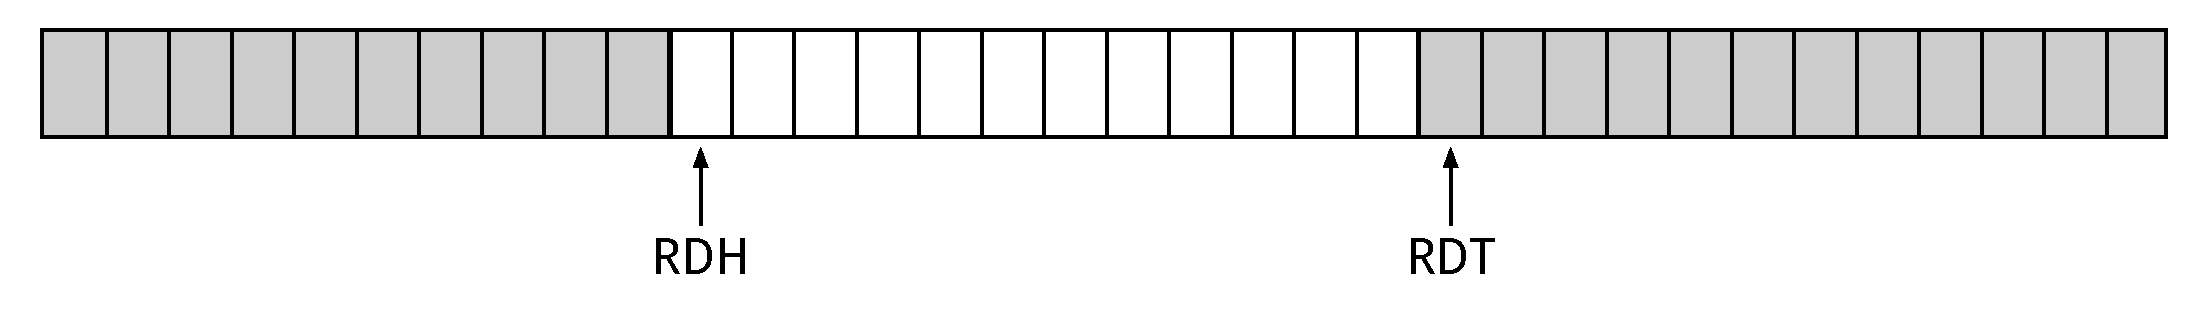
\includegraphics[scale = 0.35]{rx-ring.pdf}
\caption{The e1000 RX ring with its index registers. The grey area contains software-owned descriptors, while the white area
	contains hardware-owned descriptors.}
\label{fig:rxring}
\end{figure}


\subsection{Interrupts generation}
\label{sec:e1000int}
The e1000 network adapter can generate interrupts for different reasons.

We are interested in two types of interrupt:
\begin{itemize}
    \item TX interrupts: these interrupts are generated when the transmission of one ore more hardware-owned frames completes. Each TX 
	  descriptor has
	  a bit flag (Report Status, RS) that can be set to specify if the harware should send an interrupt as soon as the transmission 
	  of the associated
	  frame is complete. In every case an interrupt is always sent when the TX ring becames empty (TDH == TDT).
	  The interrupt routine, depending on the OS and the driver implementation, may execute cleanup operations on the descriptors 
	  that have been processed and mark them as free to be used to commit new frame to the adapter.
	      
    \item RX interrupts: these interrupts are generated after the hardware has received (and stored in physical memory) an incoming frame, 
	  in order to notify the driver that can send the frame to the kernel network stack. When the frame is sent to the kernel, it will
	  find the right way to its destination, that can be anything (trash included). Assuming the destination is a user process,
	  what the OS does is just to append the packet to a queue associated to the receiving socket. At this point the sleeping user
	  process is notified and can be scheduled to complete the read operation from the socket queue.
\end{itemize}

There is a big concern when dealing with RX interrupts. If the device doesn't limit them, they act as a source of uncontrolled load for the 
CPU.
The receiving machine, in fact, is forced to serve incoming RX interrupts even if the RX interrupt rate is very high. Since we are
dealing with high performance devices, we must be able to receive up to 1 Mpps (or even more).
The overhead involved in interrupt handling is generally quite high, and so each interrupts has a fixed cost that must be paid before
doing useful work, such as push the received frame to the network stack and let the receiver process actually receive it.

If each packet receive generated an interrupt, we would have to handle up to 1000000 interrupts per seconds, which something that would
completely stall our machine.
When the interrupt rate is too high, in fact, the machine spends almost all the time serving interrupts\footnote{The interrupt handling is
by its nature an high priority task with respect to normal process execution.}, and there is no time left for other things to happen,
e.g. for user processes to read the received packets. This is a quite bad situation, because the CPU is 100\% utilized, but the machine,
on the whole, cannot do any useful work.

The situation could be slightly better if the machine has more than one CPU, but still it's not good for the CPU servicing the interrupts
to spend too much time in interrupt handling overhead.

\vspace{0.5cm}

Cleary, this problem can only be solved if the device somehow collapses RX interrupts, raising an interrupt every batch of received
frames, let's say 100 frames per batch, and not every single frame. In this way the interrupt rate is 100 time lower, and the
interrupt overhead cost is amortized over 100 frames.
In every case the device must guarantee that a RX interrupt is eventually sent after a period of inactivity, even if it is still waiting
for a 100-frames batch to be completed, because the device cannot know when the next frames are going to come.

These and similar mechanisms are know as \emph{interrupt mitigation} or \emph{interrupt moderation}, since they tries to moderate the
interrupt rate.

Interrupt moderations is commonly applied also to TX interrupts (or to all the interrupts in general). The TX interrupt rate can be
controlled because the driver can control (and limit) the TX rate. Neverthless it is convenient for the driver to take advantage of
the interrupt-rate-limiting hardware capabilities rather than implement a similar feature in software\footnote{With e1000, an TX 
interrupt moderation mechanism could be implemented using the RS bit.}.

\vspace{0.5cm}

The e1000 class of network adapters implements two interrupt moderation mechanisms.

\subsubsection{The older moderation mechanism}
The older mechanism is supported by the registers TIDV (Transmit Interrupt Delay Value), TADV (Transmit Absolute Interrupt Delay Value),
RDTR ( and RADV, where each register is provided with a countdown timer.

\vspace{0.5cm}

TIDV and TADV, when properly set, can be used to provide TX interrupt moderation on a per-descriptor basis.

When the adapter processes a a TX descriptor, if the RS bit and the IDE bit\footnote{The Interrupt Delay Enable bit (IDE), is another
bit flag in the TX descriptor, like the RS bit.} are set, an interrupt is not raised immediately, but the TIDV timer is started (or
restarted) with the value specified in the TIDV register itself. When the TIDV timer expires, an interrupt is raised in order
to inform the driver about the TX completion of one or many frames, and the TIDV timer is cleared.
The TIDV register can therefore be used to coalesce TX interrupts.

However, it might be necessary to ensure that no completed transmission remains unnoticed for too long an interval in order to 
ensure timely release of TX buffers.
The TADV register has been added for this purpose. Like the TIDV timer, tha TADV timer only applies to TX descriptor where both the
RS bit and the IDE bit are set. This register can be used to ensure that a TX interrupt occurs before a predifined time interval
after a transmission (whatever) is completed. The time interval can be specified in the TADV register itself.
In order to do this, after each TX descriptor is processed, the TADV timer is is started (armed with the value specified in the TADV 
register) only if it is not already running.
When the timer expires, a TX interrupt is generated.

\vspace{0.5cm}

RDTR and RADV, when properly set, can be used to provide RX interrupt moderation on a per-received-frame basis.
The RDTR timer is started (or restarted) immediatly after a new packet is received and transferred to physical memory, using
the interval value specified in the RDTR register. When the RDTR timer expires, an RX interrupt is raised, and the timer is cleared.
The RDTR register can therefore be used to coalesce RX interrupts, in the very same way the register TIDV is used to coalesce TX
interrupts.

Also in the RX case it may be necessary to ensure that no receive remains unnoticed for too a long interval. The RADV register deal
with this problem, in the very same way the TADV register does, so we won't explain the mechanism again.

\vspace{0.5cm}

The figure \ref{fig:rdtrstate} shows a state diagram associated to the RDTR timer.

\begin{figure}[bt]
\centering
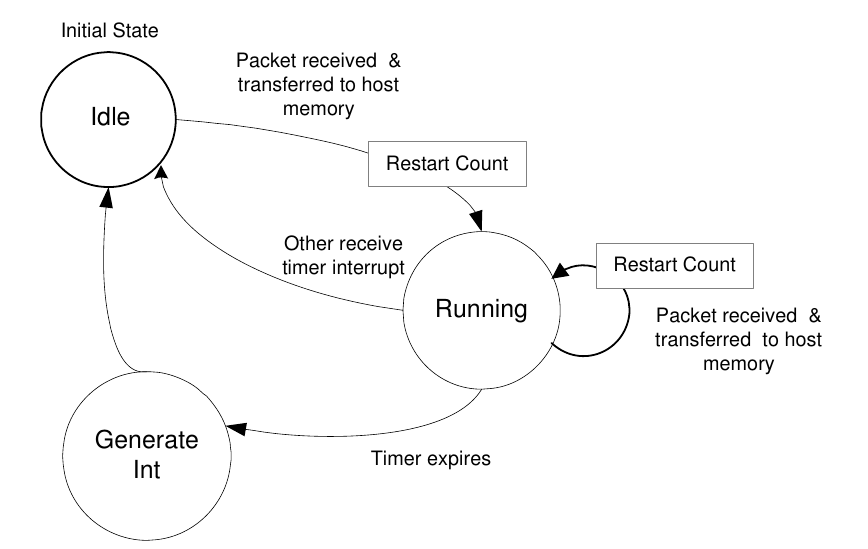
\includegraphics[scale = 0.45]{rdtr-state.png}
\caption{State diagram of the RDTR timer (Packet Delay Timer). CITE INTEL}
\label{fig:rdtrstate}
\end{figure}

The figures \ref{fig:radv} and \ref{rdtrradv} depict some examples about the RDTR and RADV moderation mechanism.

\begin{figure}[bt]
\centering
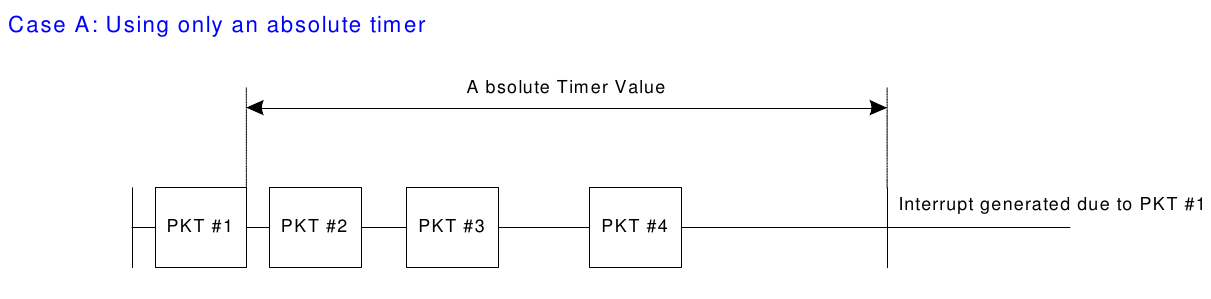
\includegraphics[scale = 0.45]{radv-only.png}
\caption{RX moderation example that makes use of the RADV timer.}
\label{fig:radvonly}
\end{figure}

\begin{figure}[bt]
\centering
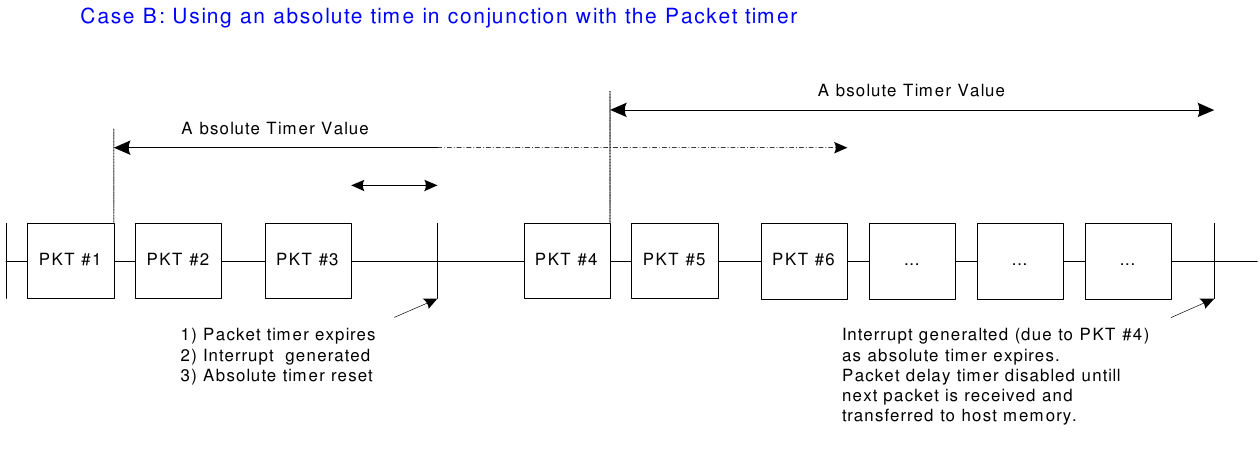
\includegraphics[scale = 0.45]{rdtr-radv.png}
\caption{RX moderation example that makes use of both RADV and RDTR timers.}
\label{fig:rdtrradv}
\end{figure}


\subsubsection{The newer moderation mechanism}
Although the older mechanisms allows for fine grained control over the moderation, expecially on the TX side, most of the times the 
required moderation functionality is way simpler. For these reason a more direct moderation mechanism has been added, which is implemented
through the ITR register (Interrupt Throttling Register).

If the driver set this register to a value $\delta$, the board ensures that $\delta$ is the minimum inter-interrupt delay, regardless of
network traffic condition, and the interrupt type.
In other words, every time an event happens that requires an interrupt (e.g. TX completion or RX completion) the board raise an interrupt
as soon as possible, while meeting the ITR inter-interrupt delay constraint.

\vspace{0.5cm}

The ITR mechanism, when used, applies to all the interrupts. The Intel manual strongly recommend avoiding the RDTR and RADV register,
and use the ITR instead.



\section{QEMU e1000 emulation}
The \emph{e1000} device is implemented in QEMU through a single source file\footnote{hw/e1000.c in the QEMU project root directory}.
This code contained in this file is also referred to as the e1000 \emph{frontend}, according to the terminology introduced in section
\ref{sec:frontback}.

A small part of this code contains declarations and routines necessary to register and initialize/uninitialize a new PCI Ethernet 
device within the rest of the emulator. In this way one or more instances of the e1000 network device can be included by the QEMU users
when launching QEMU\footnote{This is done through the \texttt{device} option. E.g. \texttt{qemu-kvm -device e1000 ...} }.

When registering a new PCI device, it is necessary to describe the I/O or MMIO regions that the device implements, registering new
PCI BAR registers. Each BAR register correspond to a different I/O or MMIO region.
When registering a new BAR, you can specify the callback functions that are invoked whenever the guest code access (reads or writes)
a location in a region.

The e1000 emulation code registers a MMIO region and an I/O region. The I/O region isn't actually used, whereas
the MMIO region maps all the registers the e1000 device implement, such as TDT, TDH, RADV, TIDV and so on.

A couple of statically defined dispatch tables, one for the read accesses and the other for the write accesses, are used to associate a
different function to each register.
In this way ones can (potentially) write a read callback and a write callback for each e1000 register.
The emulation of a device is basically achieved with this per-register functions. Of course register can share the same functions or have
no callback at all.

\vspace{0.5cm}
Let's see in more depth how register callbacks are actually invoked.

When a VCPU is executing the guest code, it may try to access a MMIO location corresponding to the e1000 PCI device, namely an e1000
register. This usually happens when executing the e1000 device driver.
The accessing instruction causes a VMExit to happen, and the VCPU thread switches from the guest world to the host world. 
After the \texttt{iothread\_lock} has been acquired, the QEMU code analyzes the VMExit reason and understands that the VMExit was caused
by a MMIO access.
It then uses the physical memory address involved by the memory access to dispatch the event to the right PCI memory region.
In our case, the read (write) callback registered with the e1000 MMIO BAR is invoked. This callback uses the address to access the 
e1000 read (write) dispatch table and invokes the specific callback associated to the accessed register.

The register-specific callback emulates the side effects associated with the register access. For instance a write to the TDT
register will cause the emulated hardware to process all the pending TX frames (see section \ref{sec:txring}).

After the callback returns, the \texttt{iothread\_lock} is released and a VMEnter is executed so that the VCPU switches back to the 
guest world.

\vspace{0.5cm}

This said, we won't describe in detail all the aspects involved in e1000 emulation. Instead, we will outline the frame
transmission and frame reception process, focusing on notifications, scheduling and memory copies.


\subsection{TX emulation}
As we wrote in section \ref{sec:txring}, a write to the TDT register is the way the driver notifies the hardware that new TX frames 
are ready to be processed.
The TDT register write callback updates the TDT value and then calls the \texttt{start\_xmit} function. This function is a while
loop that processes all the committed TX descriptors, starting from the descriptor pointed by the TDH register. After each
descriptor has been processed, the TDH register is incremented circularly. The while loop exits when TDT == TDH, e.g. there
are no more TX descriptors to be processed.

When a TX descriptor is processed, the following actions are performed:
\begin{enumerate}
    \item The TX frame corresponding to the TX descriptor is copied from the guest memory in a local buffer.
    \item The TCP/UDP checksum is computed. Recall that e1000 devices are able to compute checksums in hardware, and so the OS 
	  driver expects the emulated hardware to be able to do it.
    \item The descriptor is written back to the guest memory in order to report that the TX descriptor has been processed.
    \item The \texttt{qemu\_send\_packet} function is invoked in order to pass the frame to the network backend. With the TAP backend,
	  a \texttt{write} system call is invoked to pass the frame to the TAP device associated with the backend.
\end{enumerate}

It's very important to observe that all these operations (frontend and backend) are performed by the same VCPU thread that tried to 
execute the TDT write operation in the guest, causing a VMExit.
This means that when the guest has only a VCPU (no SMP) the emulation of a transmission cannot be done in parallel with the guest, being
done synchronously with the VCPU thread.

\vspace{0.5cm}

When all the pending TX descriptors have been processed, the interrupt pin associated with the e1000 adapter is raised (if it previous
pin state was low), sending an interrupt to the guest.


\subsection{RX emulation}
When a receiving guest is waiting for new frames to come, the IOThread is blocked in the \texttt{select} system call.
When a frame arrives to the TAP backend, the \texttt{select} returns and invokes the TAP network backend.
The backend executes a \texttt{read} system call on the TAP device, extracting the incoming frame, and invoke the \texttt{qemu\_send\_packet}
function that passes the frame to the e1000 frontend, namely to the receive method \texttt{e1000\_receive}.

According to what has been said in \ref{sec:rxring}, the \texttt{e1000\_receive} method perform the following actions:
\begin{enumerate}
    \item If RDH == RDT, there are no RX memory buffer available, and the incoming frame must be dropped.
    \item The RX descriptor pointed by the RDH register is fetched from the guest memory.
    \item The incoming frame is copied to the guest memory location at the address specified in the RX descriptor.
    \item If not already high, the e1000 interrupt pin is raised.
\end{enumerate}

Differently from the TX emulation, here all these operations (frontend and backend) are executed by the IOThread, that can run in parallel
with the VCPU thread (or the VCPU threads) executing the guest code.

\vspace{0.5cm}

When the \texttt{qemu\_send\_packet} function returns, the backends tries to read another frame from the TAP\footnote{The \texttt{read}
system call is non-blocking, since the IOThread is executing an event-loop, and so only the central \texttt{select} system call is
allowed to block.}. If there is another frame to process, the \texttt{qemu\_send\_packet} is called also on this frame.
This process stops when no frames are ready to be read from the TAP, or when the packet is dropped by the frontend.



\section{Linux e1000 device driver}
In this section we will describe some details about the e1000 device driver code in the Linux kernel.
We will only illustrate those aspects that are relevant to our goals.
The driver source code can be found in the directory drivers/net/ethernet/intel/e1000 in the Linux kernel project root directory.

\subsection{Interface with the kernel}
The Linux kernel API has a specific network API that the network device driver uses in order to exchange network packets with
the rest of the kernel.

With these API, the network driver can register a new network interface within the kernel, associating a name to it.
The list of all the network interfaces currently registered within the kernel can be seen using the \texttt{ifconfig} utility
(e.g. \texttt{\$ ifconfig -a})or similar tools.
The registering function, \texttt{register\_netdev}, requires as input argument a \texttt{netdev} structure that abstracts the
registering network adapter. This structure contains all the information necessary to the kernel to use with the adapter.

The most important fields are:
\begin{itemize}
    \item \texttt{name}, which is a string that univocally identifies the new network interface in the system.
    
    \item \texttt{netdev\_ops}, which is a structure containing the methods that the new network interface exports to the kernel 
	  (see below).
	  
    \item \texttt{watchdog\_timeo}, which specifies the minimum time interval that the kernel should wait after a transmission is commited
	  to the device driver before deciding that something could be wrong. When a transmission is committed, the watchdog timer 
	  associated with the network interface is started. When the driver knows that the hardware it done with the committed frame,
	  it release the associated TX buffer (in e1000 this can be done in the routine that handles the TX interrupt). On the release,
	  the watchdog timer is cleared. If the timer fires, the \texttt{ndo\_tx\_timeout} method is called, and the driver could
	  handle potential hardware hangs.
	  
    \item \texttt{hw\_features}, which is a bitmask that specifies to the kernel the features offered by the hardware that can be activated
	  or deactivated by the user. The e1000 device driver specifies, among the others, the \texttt{NETIF\_F\_HW\_CSUM} (checksumming
	  capability) feature, the \texttt{NETIF\_F\_SG} (scatter-gather capability) feature and \texttt{NETIF\_F\_TSO} (TCP Segmentation
	  Offload capability).
	  
    \item \texttt{features}, which is a bitmask that represent the currently active features. This mask can be initialized to the same
	  value as the \texttt{hw\_features} field, but can be modified by the users to set/unset features and fixed by the kernel in
	  order to meet feature constraints\footnote{The features are not independent on each other within the kernel.}.
	  
    \item \texttt{dev\_addr} and \texttt{perm\_addr}, which contain the hardware address of the network adapter. As far as we are
	  concerned, these two fields are set to the same value. In the e1000 adapter, the hardware address is read from an on-board
	  EEPROM.
\end{itemize}


The \texttt{netdev\_ops} contains several methods, but we are intersted only in a few ones:
\begin{itemize}
    \item \texttt{ndo\_open}, which is called when the system administrator decides to bring the network interface up. This can be done
	  using the \texttt{ifconfig} utility (e.g. \texttt{\#ifconfig eth0 up}) or similar. The driver should react to this request by
	  setting up all the resource (software or hardware) necessary for the adapter operation.
	  
    \item \texttt{ndo\_close}, which is called when the system administrator decides to bring the network interface down, This can be
	  done using the \texttt{ifconfig} utility (e.g. \texttt{\# ifconfig eth0 down} or similar. When receiving this request,
	  the driver can release all the resource necessary for the adapter operation.
	  
    \item \texttt{ndo\_start\_xmit}, which is invoked by the kernel when it wants to transmit a new frame. The first argument is
	  a pointer to a \texttt{sk\_buff} structure, which contains all the information related to the frame to transmit, including
	  the frame itself. The \texttt{sk\_buff} structure is central to the Linux kernel networking, since all the layers in the 
	  network stack perform actions on this structure.
	 
\end{itemize}

At the end of the \texttt{ndo\_open} method, if everything is ok, the driver have to call the \texttt{netif\_start\_queue} function,
that tell the kernel it can start transmitting frames through the network interface, namely can call the \texttt{ndo\_start\_xmit}
method.

\vspace{0.5cm}

On the receive side, the kernel networking API provides the network driver with a way to pass a received frame up to the network
stack, where the frame can find its way to its destination.
The frame is handed off to the network stack as a \texttt{sk\_buff} structure, since the stack only works with this kind of structures.
When receiving a frame from the adapter, therefore, the driver has to build a \texttt{sk\_buff} structure around the frame received
and call the function \texttt{netif\_rx} with the built structure as parameter, in order to hand it off to the kernel.

\begin{figure}[bt]
\centering
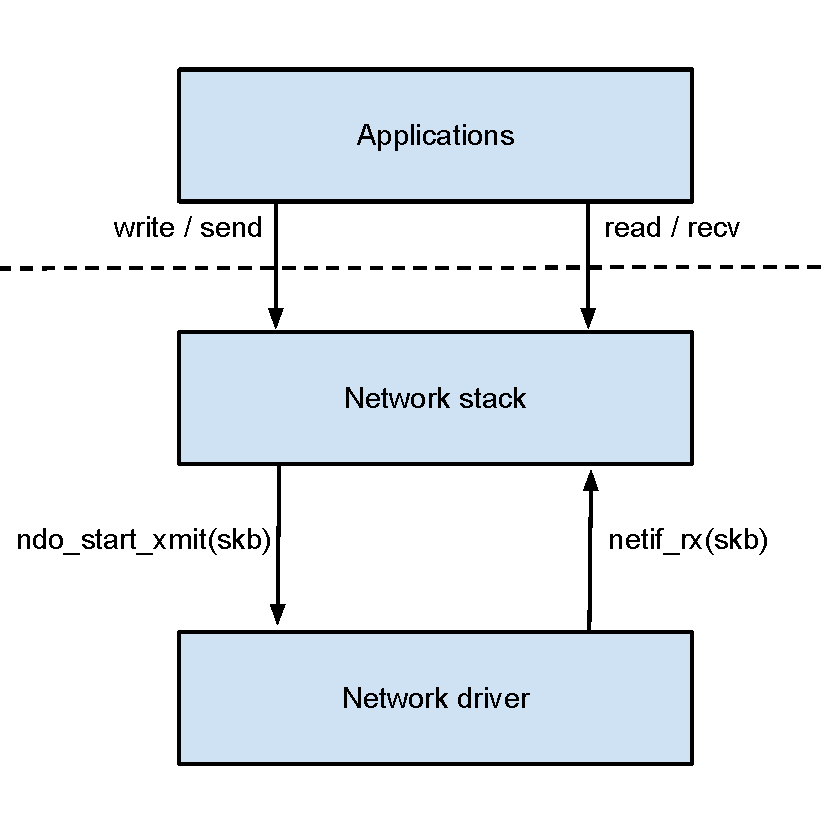
\includegraphics[scale = 0.65]{linux-interface.pdf}
\caption{On the bottom the interface between the network device driver and the network stack, and on the top the interface between
user applications and the network stack.}
\label{fig:linux-interface}
\end{figure}


\subsubsection{The NAPI interface}
The receive interface described earlier is known as the ``older'' interface. The \texttt{netif\_rx} is intended to be invoked
directly by the interrupt routine associated with an RX interrupt.

However, as we pointed out earlier (see \ref{sec:e1000int}), the RX interrupt are source on uncontrolled load and must be moderated when
the interrupt rate is too high. This can be done by hardware mechanisms, but a complementary software approach can still be useful.
Moreover, a software interrupt moderation can be fundamental if hardware moderation is not provided by the network adapter.

\vspace{0.5cm}

The software approach is based on the concept of \emph{polling}. Interrupt operation was introduced in the early days of computing when
the computer architects realized that when dealing with devices through polling most of the CPU cycles were thrown away because of
busy waiting. Interrupt operation makes it possible to avoid busy waiting, even though it carries with it a fixed overhead, due to the
context switches and scheduling operations, that is fairly high.

Nevertheless, if there is (almost) always an hardware event to handle, busy waiting is not a problem, since there is nothing to wait for.
Polling can therefore be used in situations where the input load is very high and so each time we want to check if there are more hardware
event to handle we have an high probability that the answer is positive. The big advantage of polling on interrupt operation is that the 
former does not have any overhead.

\vspace{0.5cm}

In conclusion, one cannot say in general that interrupt operation is better than polled operation or the other way around. When the hardware
event rate (e.g. frame reception rate) is low enough, it's worth paying the fixed cost associated with interrupts but be sure that there
is an event to handle. When the event rate is high enough, doing busy waiting it's cheaper than using interrupts, because the average cpu
cycles wasted for each received frame is way lower than the cpu cycles wasted for the interrupt overhead.

The NAPI (New API) interface has been designed with these considerations in mind. When a RX interrupt arrives, the driver interrupt routine
could decide to switch to polling mode, and not to handle the received frame directly in the interrupt routine.
This is done simply disabling the interrupt on the network adapter and scheduling a NAPI context. The latter action is done invoking the 
function \texttt{napi\_schedule}.
The NAPI context it's going to be executed in a kernel thread context different from the interrupt context. This is basically another form of
deferred work.

When the NAPI context is scheduled it executes the NAPI polling function registered by the driver (e.g. in the \texttt{ndo\_open} method)
through the function \texttt{netif\_napi\_add}.

The NAPI polling function has to do the receive work\footnote{or the interrupt work in general}. Of course the polling function is intended
to process more RX frames. In order to prevent the polling function to kill the CPU...

\chapter{Optimizations of emulated e1000 performance}
\label{cha:e1000-opt}
In chapter \ref{chap:env} we have given an overview of the software environment we will deal with in this work.
In this chapter we will analyze problems and bottlenecks of the current system implementation and propose solutions that are able
to remove them.

\vspace{0.5cm}

First of all we have to point out what we are going to optimize. We consider two scenarios.

In the first scenario, \emph{guest to host} (G2H), a VM is connected to the host through a host-only virtual LAN (see 
section \ref{sec:qemunet}). The VM runs an application that sends UDP packets of a given size at a given average rate, while 
the host runs an application that receives all the UDP packets it can.
The second scenario, \emph{host to guest} (H2G), is very similar to the first, but the host and guest roles are swapped: the host runs 
the UDP sender while the guest runs the UDP receiver. These scenarios are depicted in figures \ref{fig:scenario-1} and \ref{fig:scenario-2}.

Our goal is to maximize the packet rate of the application running on the VM, both on the transmit and the receive side.

\vspace{0.5cm}

In our experiments, we will try to give to each guest one or two VCPU, and discuss the differences between the two cases.

\begin{figure}[bt]
\centering
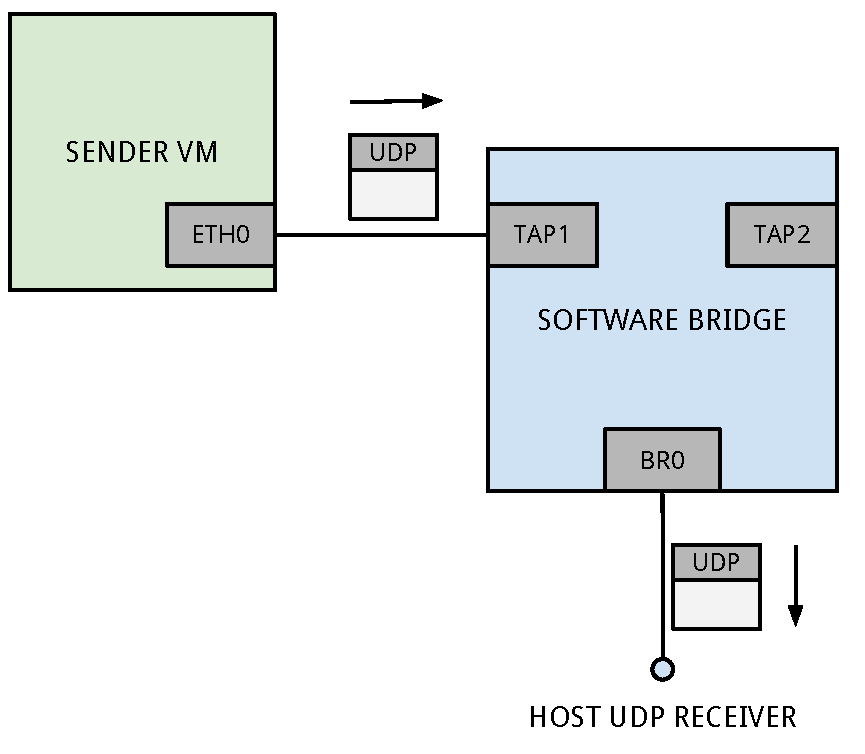
\includegraphics[scale = 0.60]{scenario-1.pdf}
\caption{Communication scenario in which and UDP sender on a VM communicates with and UDP receiver on the host.}
\label{fig:scenario-1}
\end{figure}

\begin{figure}[bt]
\centering
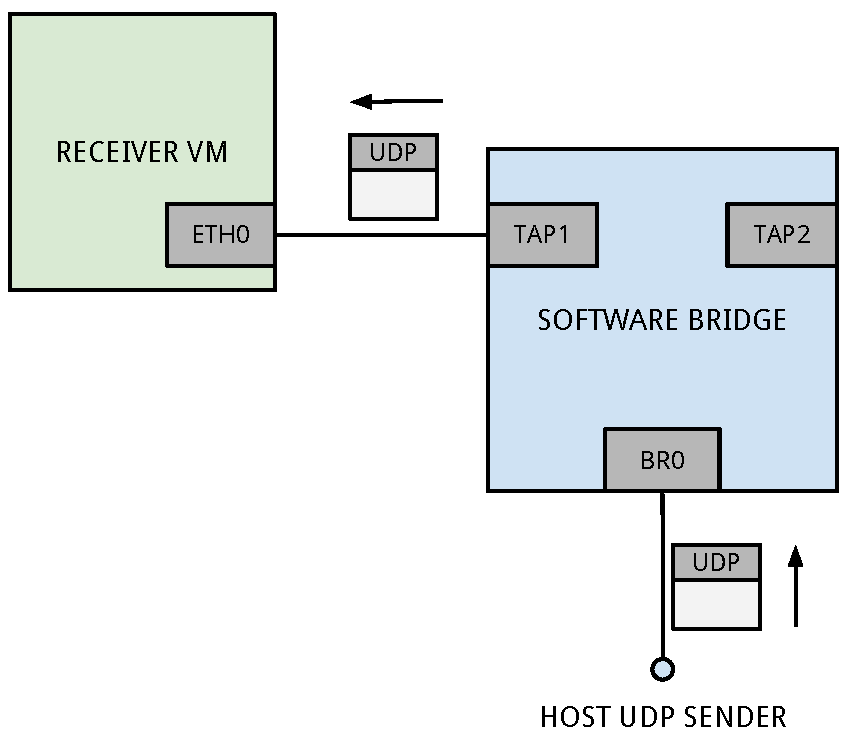
\includegraphics[scale = 0.60]{scenario-2.pdf}
\caption{Communication scenario in which and UDP sender on the host communicates with and UDP receiver on the VM.}
\label{fig:scenario-2}
\end{figure}


\section{Analysis of the existing implementation}
\label{sec:e1000perf}
We are now going to show and discuss the performance of the existing solution, e.g. of the machanisms illustrated in section 
\ref{sec:e1000emu} and \ref{sec:e1000driver}.
All the measurements have been done on a laptop machine with an i5-2450M processor, which is endowed with four cores running at 
2.5GHz\footnote{The linux CPU frequency manager has been used to set the CPU frequency at the maximum frequency.}.

\subsection{TX performance}
\label{sec:e1000txperf}
In this experiment a VM runs an UDP sender that sends UDP packets to an UDP receiver that runs on the host. The sender is just an 
infinite loop where each iteration invokes the \texttt{send} system call. The buffer passed to the system call is always the same and its
length is such that a minimum size ethernet frame (60 bytes) is sent on the wire for each \texttt{send}.
With this test we push to the limit the TX performances in the short packet case.


\subsubsection{1 VCPU test}
\label{sec:e1000-tx-g2h1vcpu}
The measurement results are shown in the table \ref{tab:e1000-tx-g2h1vcpu}. The guest has been assigned 1 VCPU, and all the values are
computed counting the number of occurrences of each event over a 1 second period and then dividing the count by the period itself.

\begin{table}
\begin{center}
\begin{tabular}{lrl}
\toprule
\textbf{Interrupt rate} & 20.567 & KHz\\
\textbf{TX packet rate} & 20.567 & Kpps\\
\textbf{TX bitrate} & 14.973 & Mbps\\
\textbf{TX notifications rate} & 20.567 & KHz\\
\textbf{MMIO write rate} & 61.702 & KHz\\
\textbf{MMIO read rate} & 61.702 & KHz\\
\bottomrule
\end{tabular}
\end{center}
\caption{Guest to host statistics with 1 VCPU per guest}
\label{tab:e1000-tx-g2h1vcpu}
\end{table}

As we can see, the TX rate is very modest, about 20.5 Kpps. There is a TX notification (a write to the TDT register) and a TX interrupt for 
each packet sent. The total number of MMIO accesses is 6 times the number of interrupts.

The high MMIO access rate is due to the interrupt routine. 
When invoked, in fact, the interrupt routine has to VMExit at least 5 times:
\begin{enumerate}
    \item Read the ICR (Interrupt Cause Read) register, in order to get the Interrupt reason (if any).
    \item Write to the IMC (Interrupt Mask Clear) register, in order to disable the e1000 interrupts.
    \item Read from the STATUS register, in order to flush the previous register write.
    \item After the NAPI work is completed, write to the IMS (Interrupt Mask Set) register in order to enable the interrupts.
    \item Read form the STATUS register, in order to flush the previous register write.
\end{enumerate}

The sixth MMIO access per interrupt is due to the TX notification.

\vspace{0.5cm}

Even if the hardware interrupt moderation is not emulated, the Linux e1000 driver uses the NAPI interface (section \ref{sec:napi}), so 
a software interrupt
moderation is actually implemented. Unfortunately, it doesn't work for TX interrupts, and the reason for this is actually very simple.
In section \ref{sec:e1000txemu} we have seen that the TX emulation is done in a synchronous way, that is the VCPU thread that writes
the to TDT register, after the VMExit, executes the e1000 frontend, the TAP backend and raises the interrupt pin. After that
it does a VMEnter coming back to the guest world, but with a TX interrupt to handle. Since the guest
has only a VCPU, the VCPU must be used to handle the interrupt, and cannot be used to insert more TX frames into the ring (e.g. to call
the \texttt{ndo\_start\_xmit} method). Consequently, the NAPI polling function will only clean the TX descriptor(s) associated to the
frame that has just been sent.
In conclusion, if we write to the TDT register every time the \texttt{ndo\_start\_xmit} method is invoked, we are doomed to receive
an interrupt for each frame we send, and so to have low performances.


\subsubsection{2 VCPUs test}
The same experiment has been done assigning 2 VCPU to the guest. The measurement results are shown in the table \ref{tab:e1000-tx-g2h2vcpu}.

\begin{table}
\begin{center}
\begin{tabular}{lrl}
\toprule
\textbf{Interrupt rate} & 23.577 & KHz\\
\textbf{TX packet rate} & 30.400 & Kpps\\
\textbf{TX bitrate} & 22.131 & Mbps\\
\textbf{TX notifications rate} & 30.400 & KHz\\
\textbf{MMIO write rate} & 61.916 & KHz\\
\textbf{MMIO read rate} & 47.274 & KHz\\
\bottomrule
\end{tabular}
\end{center}
\caption{Guest to host statistics with 2 VCPU per guest}
\label{tab:e1000-tx-g2h2vcpu}
\end{table}

Compared with the 1-VCPU case, the situation is slightly better, but still modest. Here we have about 30 Kpps, and an interrupt rate
that is significantly less than that. This means that the TX interrupt routine (e.g. the polling function), on average, handles more than
one frame.
Note that there is still only one TX frame sent for each TX notification, like in the 1-VCPU case.
The improvement is due to the higher degree of parallelism in the guest, that allows the NAPI to coalesce some interrupts, so that
on average about 1.29 data TX descriptors are cleaned for each interrupt. This happens because while one VCPU is executing the interrupt
routine (or the NAPI context is active) with the e1000 interrupts disabled, the other VCPU can find the time to insert another TX frame
in the ring, execute the frontend and backend and return to the guest without raising an interrupt because they are disabled.
This is why, sometimes, the NAPI polling function cleans more than one data TX descriptor.


\subsubsection{Discussion}
\label{sec:e1000txperfdiscuss}
The low performance is basically due to two problems: The hardware interrupt moderation is not emulated in QEMU and there is a TX 
notification for each frame to send. This is true in both 1-VPCU and 2-VCPU cases.

If we coalesced the interrupts, we could amortize the 5 VMExits and the interrupt overhead over more TX frames.
Implementing the emulation of the hardware interrupt is then then an optimization we can implement.

If we had a way to coalesce the TX notifications we could amortize the cost of a notification over more TX frames. This
a second optimization we can implement.

\vspace{0.5cm}

We've not discussed the performances with bigger packet sizes, because the problems involved are exactly the same. When the packets are 
big there is more work to do because the packet copies are more expensive, and so the performance are lower. However,
the optimization are very effective also for the big packet case, because the overhead due to the copies is significantly lower than
the overheads due to TX notifications and interrupts.



\subsection{RX performance}
In this experiment a VM runs an UDP receiver that receives UDP packets from an UDP sender that runs on the host. The receiver is just an 
infinite loop where each iteration invokes the \texttt{recvmsg} system call. No processing is made on the received packet.
The UDP sender is similar to the sender used in section \ref{sec:e1000txperf}, but after each \texttt{send} system call the process
does some busy waiting in order to send UDP packets at a given rate.
With this test we push to the limit the guest RX performances in the short packet case.

\vspace{0.5cm}

The receiving process is generally more problematic than the transmit process, because of the \emph{livelock} problem (see section 
\ref{sec:e1000int}).
When the incoming packet rate and/or the interrupt rate are too high, or the traffic is very irregular with high traffic peaks, the guest
OS (device driver and network stack) does a lot of processing before trying to put the packet in a socket receive queue, but in the end
is forced to throw them away because the queue is full. In its turn, the queue is full because the receiver process doesn't have enough
time to read all the packets from the queue.

\vspace{0.5cm}

For this reason we introduce the concept of (receiver) \emph{critical} rate. We define the critical rate as the incoming packet rate that,
if exceeded, cause the receiver VM to enter a unstable state and/or a state characterized by bad performance. In more detail, in our
experiment we will see the RX rate measured by the UDP receiver as a function of the RX rate measured by the network adapter (the incoming 
rate).
When the incoming rate is low enough, the UDP receiver will measure the same rate, because no packets are dropped. As the incoming rate gets
higher a little percentage of packets starts to be dropped, and so the UDP-measured rate is a little lower than than the incoming rate, but
still increases when the incoming rate increases. When the incoming rate exceeds the critical rate, however, the UDP-measured rate starts
to decrease when the incoming rate increases. Moreover, beyond the critical rate the UDP-measured rate generally oscillates, e.g. the
receive system becomes unstable and its responsiveness becomes very low.
Figure \ref{fig:cr} shows an example of the function we are talking about.

\begin{figure}[bt]
\centering
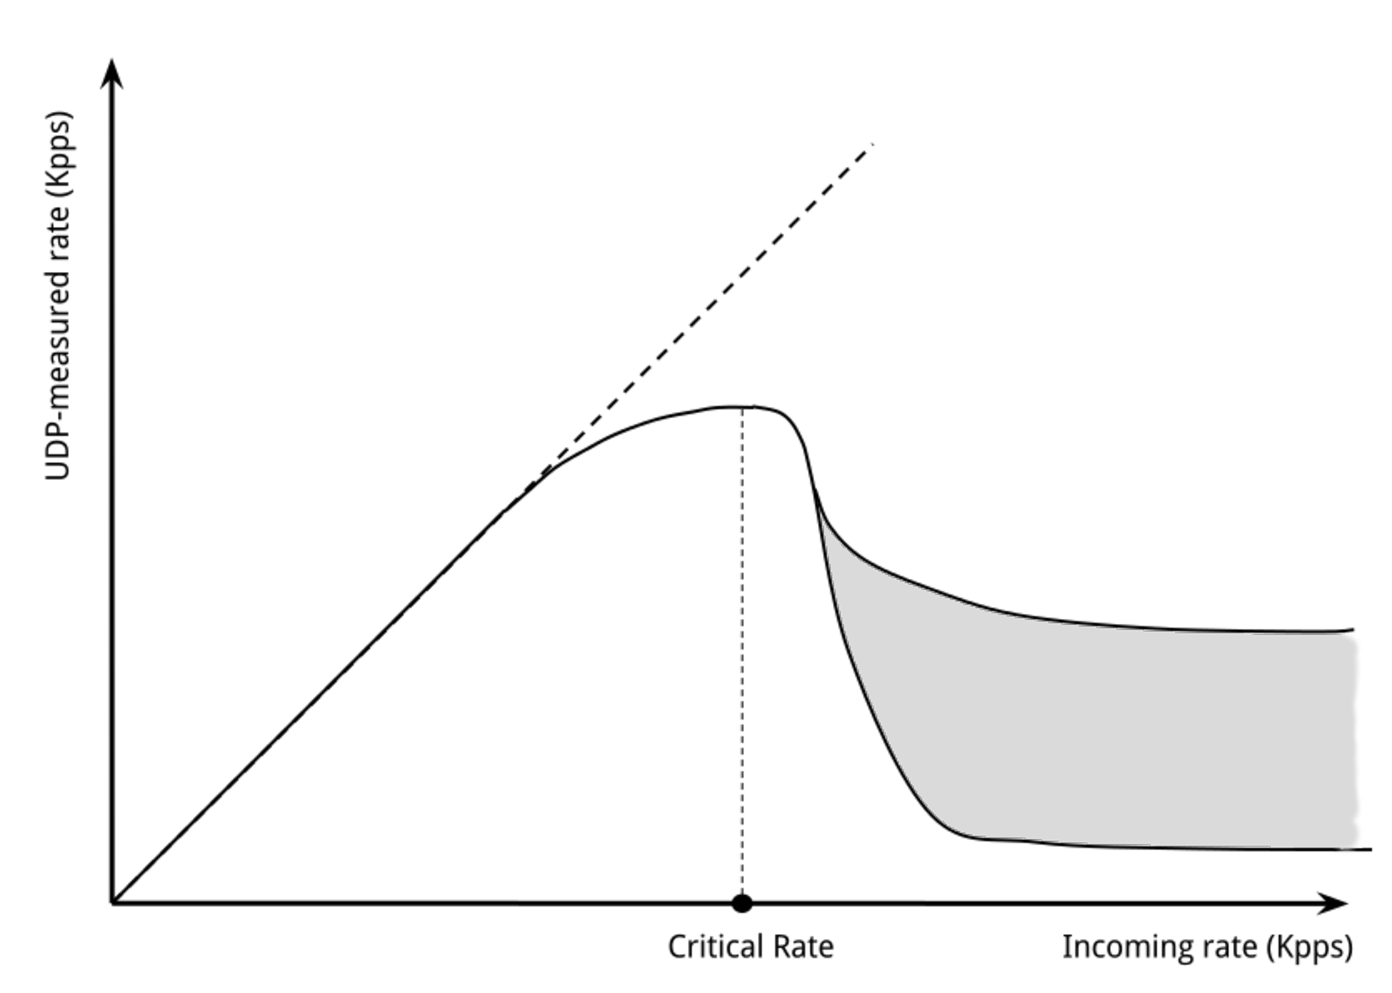
\includegraphics[scale = 0.55]{critical-rate.pdf}
\caption{This plot is an example the RX rate measured by the UDP receiver as a function of the RX rate measured by the network adapter.
	 The critical rate is the incoming rate for which this function has a maximum. The gray area represent the oscillation (upper and
	 lower bound) of the UDP-measured RX rate.}
\label{fig:cr}
\end{figure}

\vspace{0.5cm}

The critical rate is very significant, since it tells what is the maximum incoming rate that a guest OS running simple receiver process can
accept while being in a stable state.


\subsubsection{1 VCPU test}
\label{sec:e1000-rx-g2h1vcpu}
In this test one VPCU is assigned to the guest. The measured critical RX packet rate is about 14.4 Kpps.
The measurement results shown in table \ref{tab:e1000-rx-g2h1vcpu} are taken when the received rate is about the same as the critical
rate.

\begin{table}
\begin{center}
\begin{tabular}{lrl}
\toprule
\textbf{Interrupt rate} & 14.314 & KHz\\
\textbf{RX packet rate} & 14.403 & Kpps\\
\textbf{RX bitrate} & 10.485 & Mbps\\
\textbf{RX notifications} & 14.288 & Mbps\\
\textbf{MMIO write rate} & 42.861 & KHz\\
\textbf{MMIO read rate} & 42.860 & KHz\\
\bottomrule
\end{tabular}
\end{center}
\caption[H2G with 1VCPU per guest]{Host to guest statistics with 1 VCPU per guest}
\label{tab:e1000-rx-g2h1vcpu}
\end{table}

The critical RX rate is very low. If we keep incrementing the incoming RX rate beyond the critical point, the system enters a livelock 
state. Since more RX interrupt work is requested and we only have a VCPU, the receiver user process has less CPU time than before, even
if there are more packets to receive. As a result, the RX throughput seen by the user process drops immediately after the critical rate,
the system become extremely instable, and most of the packets are dropped. With packet rates higher than 15 Kpps the system becomes
unusable.

\vspace{0.5cm}

Let's analyze what happens when the livelock doesn't shows up (table \ref{tab:e1000-rx-g2h1vcpu})
The interrupt rate is a little lower than the RX packet rate, and this means that some interrupts have been coalesced by the NAPI.
This is possible even with a single VCPU, differently from what happens int the TX case, because (see section \ref{sec:e1000rxemu})
the hardware emulation (backend and frontend) is done by the IOThread, while the guest is executed by a VCPU thread. Parallelism is 
therefore possible, because the IOThread could insert a new frame in the RX ring while the NAPI is polling, and/or the interrupt could
be delayed because the interrupts are disabled.

However, the two rates are almost the same, and so we still have approximately an interrupt for each frame received, which means that
the NAPI software moderation isn't not working well. More precisely, we have measured the distribution of the amount of RX NAPI work
done each time the polling function is called and reported it in table \ref{tab:e1000-rx-napi-dist}.

\begin{table}
\begin{center}
\begin{tabular}{lrl}
\toprule
\textbf{NAPI RX work} & \textbf{Percentage}\\
\midrule
0 & 0.05\%\\
1 & 99.485\%\\
2 & 0.335\%\\
$\geq$ 3 & 0.13\%\\
\bottomrule
\end{tabular}
\end{center}
\caption{Host to guest NAPI distribution with 1 VCPU per guest. The NAPI work is the number of
frames handled by the execution of the polling function.}
\label{tab:e1000-rx-napi-dist}
\end{table}

\vspace{0.5cm}

Why is the NAPI working so bad? The problem here isn't related to lack of parallelism, like in the TX case, but is due to the guest being
too fast. In fact, we can observe that in this experiment the overall system is composed of a \emph{producer} thread, e.g. the IOTHread,
and a \emph{consumer} thread, e.g. the VCPU thread. The producer is basically an infinite loop that in each iteration gets a frame from the
TAP (waiting/sleeping if no frames are ready to be read),
inserts it in the RX ring and raises an interrupt if enabled. The consumer is woken up by an interrupt and schedules the NAPI context.
The NAPI polling functions is a loop that on each iteration extracts an RX frame from the ring and push it to the stack, until there is no
work left.

If the consumer iteration is on average slower than the producer iteration, the latter is very likely to find the interrupts disabled
after inserting a new RX frame, and the consumer is very likely to see the new frame while is executing the polling function corresponding
to a previous interrupt. In this scenario the consumer will (almost) always find work to do, and so the interrupt will (almost) always
be disabled, and consequently the NAPI mitigation will work.

On the other hand, if the consumer iteration is on average faster than the producer iteration, the latter is very likely to find the
interrupt enabled after inserting a new RX frame, and so an interrupt is raised for each received frame. This is exactly what happens
in our experiment. It's important to point out that when there is no more work to do, the NAPI polling function is forced to complete 
and enable the interrupts, because it doesn't know when the next RX frame is going to come.

Observe that in this experiment the consumer is very slow simply because we have forced the UDP sender to send to a 
constant packet rate of 14 Kpps, which makes it slow by definition. We cannot go beyond 14Kpps because of the livelock.

\vspace{0.5cm}

Moreover, as we can see in the table \ref{tab:e1000-rx-g2h1vcpu}, we also have approximately a write to the RDT register (RX 
notification) for each interrupt, which is not good. This is also a consequence of the NAPI misbehaving.

Similarly to the 1-VCPU TX case, here we have 6 MMIO accesses for each interrupt. Five of them are exactly the same listed in
section \ref{sec:e1000-tx-g2h1vcpu}, while the sixth one correspond to the RX notification.


\subsubsection{2 VCPUs test}
The same experiment has been done assigning 2 VCPU to the guest. Here the critical rate is way higher, about 175 Kpps. Moreover,
if the rate is passed, the system still works, even if packets start to be dropped and it becomes unstable (the dropping percentage
varies very much between 5\% and 85\%). The performances don't drop immediately after the critical rate, like in the 1-VCPU case: The system
is still usable (but not stable) if the incoming RX rate is about 300K.

The measurement results are shown in the table \ref{tab:e1000-rx-g2h2vcpu} when the incoming packet rate is about 185 Kpps.

\begin{table}
\begin{center}
\begin{tabular}{lrl}
\toprule
\textbf{Interrupt rate} & 6.696 & KHz\\
\textbf{RX packet rate} & 185.657 & Kpps\\
\textbf{RX bitrate} & 135.158 & Mbps\\
\textbf{RX notifications} & 13.725 & Mbps\\
\textbf{MMIO write rate} & 22.661 & KHz\\
\textbf{MMIO read rate} & 13.459 & KHz\\
\bottomrule
\end{tabular}
\end{center}
\caption[H2G with 2VCPU per guest]{Host to guest statistics with 2 VCPU per guest}
\label{tab:e1000-rx-g2h2vcpu}
\end{table}

As we can see, here the NAPI works very well, since the producer here is way faster than 14 Kpps (see section \ref{sec:e1000-rx-g2h1vcpu}).
On average we serve about 27 RX frames per interrupt, so that the high interrupt overhead and the MMIO accesses are amortized.

The RX notification rate is about twice as the interrupt rate, because when the polling function handles more frames, it gives new memory
buffers to the hardware doing a write to the RDT register every 16 frames handled (see section \ref{sec:rxdriver}) and a write at the end
of the polling function. Since on average 27 frames are served, we have on average $\lfloor \frac{27}{16} \rfloor + 1 = 2$ RDT writes.


\subsubsection{Discussion}
The low performance in the 1-VCPU case is basically due to two problems: The hardware interrupt moderation is not emulated in QEMU and
there is a RX notification for each frame to send. The interrupt moderation here is necessary, because the NAPI mitigation doesn't work
(because of the livelock).

In the 2-VCPU case the mitigation can still be useful to remove the existing fluctuations in the interrupt rate which cause performance
drops, and in general would be useful for the system to be more stable. In our experiment, in fact, we noted that the performance drops
when the interrupt rate has a peak (~10 KHz).

The second problem has minor negative effects on performance in the 2-VPCU case, because an RX notification is done every
16 frames, so the associated cost is amortized.

\vspace{0.5cm}

We've not discussed the performances with bigger packet sizes, for the same reasons explained in \ref{sec:e1000txperfdiscuss}.



\section{Implementing interrupt moderation}
\label{sec:e1000-mit}
In section \ref{sec:e1000txperf} we have seen that we can improve both the RX and TX packet rate if we emulate the e1000 mitigation.
A precise emulation is not necessary nor possible, and it's therefore convenient to choose a simple and efficient one.
In this work we have implemented the ITR register, the TADV register and the RADV register.
We are not interested in the TIDV and RDTR registers\footnote{However, the RDTR register has been added to the frontend only to 
validate the RADV content. The e1000 speicification, in fact, says that the TADV register is not valid if RDTR contains 0.}.

\vspace{0.5cm}

In our implementation we use a single QEMUTimer (see section \ref{sec:qemuel}), even if the hardware has multiple timers, and so we have to 
aggregate the meanings and functionalities of the ITR, TADV and RADV registers.
We therefore consider the moderation delay to be the minimum delay among the ones specified through the ITR, TADV and RADV registers.
When computing the minimum, each register is considered only if its content is valid and if there is a pending event of the proper type.
According to the e1000 specification (\cite{ref:e1000}), a zero value means that the register content is not valid. If there is no pending 
TX event the TADV content is not considered, while if there is no pending RX event the RADV register is not considered.

Moreover, only the interrupts due to transmission (\texttt{start\_xmit()} function) and reception (\texttt{e1000\_receive()}
function) are considered. The other interrupts are extremely rare, so they are not intersting.


\vspace{0.5cm}
Let's see how moderation is implemented. We have modified the code so that the frontend calls the \texttt{mit\_set\_ics()} function instead
of the \texttt{set\_ics()} function when it wants to issue an interrupt.
When called with the moderation timer (\texttt{mit\_timer}) inactive, the \texttt{mit\_set\_ics()} arms the timer with the moderation delay
and issues  an interrupt.
When called with the moderation timer active (e.g. the timer has not expired yet), it only accumulates the interrupt cause, but don't issue 
an interrupt.
When the timer expires, an interrupt is sent, and the timer is rearmed only if there is a pending accumulated interrupt cause and
the moderation delay is not zero.
Every time the timer is (re)armed the moderation delay is computed again, because the mitigation registers content can change, and
the pending events could be only RX or only TX events.

In this way we are sure that the minimum inter-interrupt interval is always greater or equal than the moderation delay.

\vspace{0.5cm}

The proposed moderation patch adds about 50 lines of code to the e1000 frontend (hw/e1000.c).

\vspace{0.5cm}

In the following sections we will repeat the same experiments presented in section \ref{sec:e1000perf} in order to see the improvements
obtained with the the moderation patch. With this experiment the Linux e1000 module has been loaded specifying the following parameters:
\begin{center}
\begin{tabular}{ll}
\toprule
\textbf{Parameter} & \textbf{Value}\\
\midrule
TxIntDelay & 0\\
TxAbsIntDelay & 0\\
InterruptThrottleRate & 4000\\
\bottomrule
\end{tabular}
\end{center}

In this way we only use the new moderation mechanism (e.g. ITR). It's not necessary to specify the parameters relative to RDTR and
RADV, since RDTR is 0 by default (so both RDTR and RADV are disabled). The InterruptThrottleRate parameter actually specifies the Maximum
Allowed Interrupt Rate (MAIR), which is inversely proportional to the value that the driver has to put in the ITR register in order to limit
the interrupt rate.

\subsection{TX performance}
\label{sec:e1000-mit-tx}
The results in the 1-VCPU case is shown in table \ref{tab:e1000-mit-tx-g2h1vcpu}.

\begin{table}
\begin{center}
\begin{tabular}{lrl}
\toprule
\textbf{Interrupt rate} & 3.805 & KHz\\
\textbf{TX packet rate} & 47.849 & Kpps\\
\textbf{TX bitrate} & 34.834 & Mbps\\
\textbf{TX notifications rate} & 47.849 & KHz\\
\textbf{MMIO write rate} & 55.464 & KHz\\
\textbf{MMIO read rate} & 11.478 & KHz\\
\bottomrule
\end{tabular}
\end{center}
\caption{Guest to host statistics with 1 VCPU per guest when interrupt moderation is implemented.}
\label{tab:e1000-mit-tx-g2h1vcpu}
\end{table}

As we can see from the table, there is an important improvement. The interrupt rate is less than 4 KHz, and this is what we expected to see
since we have set the MAIR to 4000.
With reference to the existing implementation (section \ref{sec:e1000-tx-g2h1vcpu}, we have a performance gain of 2.32, with about 47 Kpps.
Since the interrupts are coalesced by the interrupt moderation mechanism, the NAPI polling function cleans on average 12.58 TX data 
descriptors each time is called. Remember that the TX emulation is synchronous with the guest VPCU (see section\ref{sec:e1000txperf}), and
so the NAPI software moderation it's useless by itself.

Despite of the good improvements, we still have a TX notification for each frame sent, and the performances are greatly limited by this
problem.

\vspace{0.5cm}

In order to understand the mitigation effects on performances, we have tried different MAIR values, computing the average TX packet 
rate on a very long time window (some minutes). The results are shown in figure \ref{fig:itr-vs-txrate}.
From this plot we can see that the lower the MAIR is, the higher the TX packet rate is. However we cannot set MAIR to a value too low,
because this would increment the latency too much. In fact while the moderation timer is on, we don't let the emulated hardware raise
any interrupt, and so the responsiveness is limited by the moderation delay, namely by the ITR.
As stated previously, in this study we want to maximize the packet rate, and we are not interested in minimizing the latency.

\begin{figure}[bt]
\centering
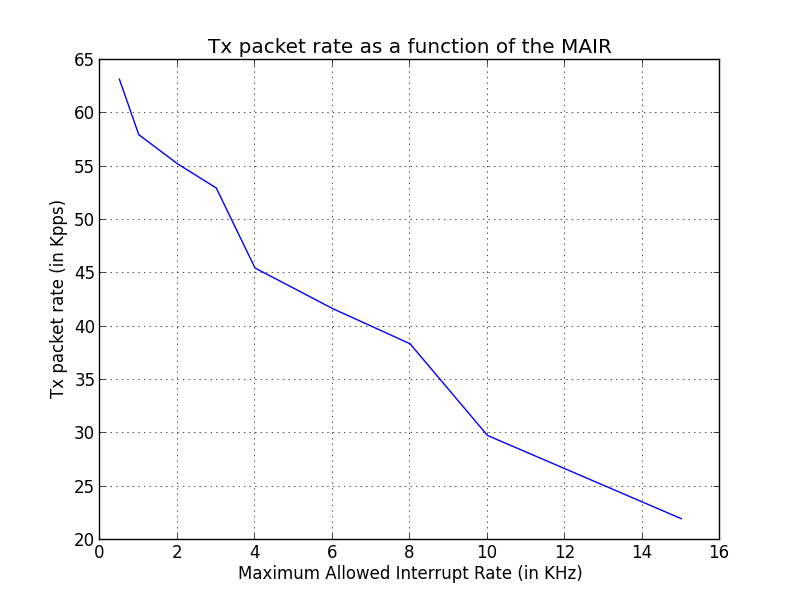
\includegraphics[scale = 0.7]{MAIR-vs-TXRate.png}
\caption{Measured TX rate as a function of the Maximum Allowed Interrupt Rate.}
\label{fig:itr-vs-txrate}
\end{figure}

\vspace{0.5cm}

The measured results in the 2-VCPU case are shown in table \ref{tab:e1000-mit-tx-g2h2vcpu}.

\begin{table}
\begin{center}
\begin{tabular}{lrl}
\toprule
\textbf{Interrupt rate} & 3.806 & KHz\\
\textbf{TX packet rate} & 47.169 & Kpps\\
\textbf{TX bitrate} & 34.339 & Mbps\\
\textbf{TX notifications rate} & 47.169 & KHz\\
\textbf{MMIO write rate} & 54.778 & KHz\\
\textbf{MMIO read rate} & 11.469 & KHz\\
\bottomrule
\end{tabular}
\end{center}
\caption{Guest to host statistics with 2 VCPU per guest when interrupt moderation is implemented.}
\label{tab:e1000-mit-tx-g2h2vcpu}
\end{table}

The results are similar to the 1-VCPU case, because the incremented parallelism is not exploited. Even if there is parallelism
between the interrupt routine and the transmission path, the TX clean work is not very expensive. Therefore we don't benefit from a second 
VCPU, or the little benefits are compensated by the overhead involved in the SMP management (e.g. locks and barriers).


\subsection{RX performance}
The measured critical rate with 1-VCPU is about 150 Kpps.
The table \ref{tab:e1000-mit-rx-g2h1vcpu} shows the results obtained when the incoming RX rate is about 137 Kpps.

\begin{table}
\begin{center}
\begin{tabular}{lrl}
\toprule
\textbf{Interrupt rate} & 3.838 & KHz\\
\textbf{RX packet rate} & 137.103 & Kpps\\
\textbf{RX bitrate} & 99.811 & Mbps\\
\textbf{RX notifications} & 10.322 & Mbps\\
\textbf{MMIO write rate} & 17.990 & KHz\\
\textbf{MMIO read rate} & 11.502 & KHz\\
\bottomrule
\end{tabular}
\end{center}
\caption{Host to guest statistics with 1 VCPU per guest, when interrupt moderation is implemented.}
\label{tab:e1000-mit-rx-g2h1vcpu}
\end{table}

As we can see, there is a huge improvement in the packet rate performance, because on average we amortize the interrupt related overhead
over about 35 frames. Since the interrupt rate is lower, also the RX notification rate is lower. On average we should expect 
$\lfloor \frac{35}{16} \rfloor + 1 = 3$ RDT writes for each interrupt (see section \ref{sec:rxdriver}), and so a notification rate of 
about $3 \cdot 3.838$ KHz = 11.514 KHz, which is similar to the measured one (10.332 KHz).

If we increase the incoming RX rate, the performance of the UDP receiver gradually degrades, but we don't run into a complete livelock 
(like the livelock we have seen in section \ref{sec:e1000-rx-g2h1vcpu}), because the interrupt rate is bounded.

\vspace{0.5cm}

In order to understand the mitigation effects on performances, we have tried different MAIR values, measuring the critical rate for
each value. The measurements are shown in figure \ref{fig:itr-vs-cr}.
The plot shows that if we increase the MAIR in in the region [2 KHz, $+\infty$], the performances gradually decrease, since we are 
less and less restrictive on the Maximum Allowed Interrupt Rate.
On the other end, if we decrease the MAIR below 1.5 KHz, the throughput starts to decrease, because the RX ring gets full and the guest
is not notified in a timely manner.
Moreover, we cannot choose the MAIR to be too low because of the latency (see section \ref{sec:e1000-mit-tx});

\begin{figure}[bt]
\centering
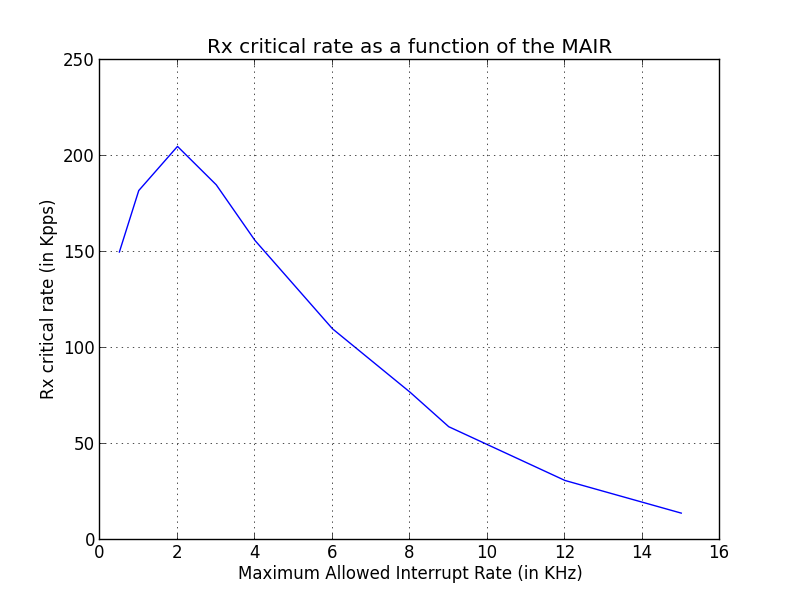
\includegraphics[scale = 0.7]{MAIR-vs-CR.png}
\caption{Measured critical rate as a function of the maximum allowed Interrupt Rate.}
\label{fig:itr-vs-cr}
\end{figure}


\vspace{0.5cm}

The 2-VCPU case results (MAIR = 4 KHz) are shown in table \ref{tab:e1000-mit-rx-g2h2vcpu}

\begin{table}
\begin{center}
\begin{tabular}{lrl}
\toprule
\textbf{Interrupt rate} & 2.098 & KHz\\
\textbf{RX packet rate} & 216.674 & Kpps\\
\textbf{RX bitrate} & 157.739 & Mbps\\
\textbf{RX notifications} & 14.321 & Mbps\\
\textbf{MMIO write rate} & 18.511 & KHz\\
\textbf{MMIO read rate} & 6.285 & KHz\\
\bottomrule
\end{tabular}
\end{center}
\caption{Host to guest statistics with 1 VCPU per guest, when interrupt moderation is implemented.}
\label{tab:e1000-mit-rx-g2h2vcpu}
\end{table}

Similarly to what happens without moderation, a second VCPU improves the RX performance, because the improved parallelism makes the
NAPI moderation to play an active role.
The measured critical rate is about 215 Kpps (+37\% w.r.t. 1-VCPU case).
We can see that the NAPI mitigation is effective observing that the average interrupt rate is half part of the MAIR, and so the MAIR is not
restrictive at operating speed. On average we have about 103 RX frames served for each interrput, which a very good result.
The expected average RX notification rate is $(\lfloor \frac{103}{16} \rfloor + 1) \cdot 2.098$ Khz = 14.686 KHz, which is very similar to
the measured result (14.321 KHz).




\section{Implementing TDT write batching}
In section \ref{sec:e1000-mit} we have seen how RX/TX packet rate performances can be improved with a minimal patch to the
e1000 frontend that implements an interrupt moderation mechanism.
However, the TX notification problem still exists and limits TX performances. The interrupt moderation mechanism cannot help to mitigate
this problem. For these reasons, we propose a TDT \emph{write batching} algorithm, which will be explained in the following section.


\subsection{Implementation}
A simple approach would be to coalesce TX notification using a counter variable. The counter is initialized to zero and is incremented 
every time the \texttt{ndo\_start\_xmit} method is invoked. A TDT write is done to notify the pending transmission only when the counter 
reaches a threshold, e.g. 20. Each time we notify we also set the counter to 0.
In this way we are able to reduce the TX notification rate by 20 times.
Unfortunately this approach would stop working when the guest stop transmitting, because we don't have a way to timely notify pending 
transmits, if any. Moreover, the \texttt{ndo\_xmit\_method} cannot know when it will be invoked again in the future. 
For these reasons we should use a kernel timer in order to notify pending transmit after a period of TX inactivity. This timer should be
(re)armed every time we don't notify, and so 19 times over 20. This is quite expensive.
Moreover, the user should have to choose the threshold value and the timer delay value, and this would add complexity and discourage the
users.

In order to get to a zero-configuration and simple implementation we have adopted an other approach.

\vspace{0.5cm}

The idea is to use the interrupt itself as a timer mechanism, and thus the interrupt routine as a timer callback.
We use a variable, \texttt{bat\_pending}, which is 1 to indicate that there is a pending interrupt that will come soon, and is
0 when there is not a pending interrupt. The variable is initialized to 0.
When the \texttt{ndo\_xmit\_method} is called for the first time, \texttt{bat\_pending} is 0: The notification is done and 
\texttt{bat\_pending} is set to 1.
If the \texttt{ndo\_xmit\_method} is called again before the TX interrupt (due to the previous notification) comes, \texttt{bat\_pending}
is 1: In this case we don't notify, and consequently that transmission become pending.
When the interrupt comes, at the begin of the NAPI polling function (the interrupt are disabled), if there are pending transmissions we do 
a notification, but we don't set \texttt{bat\_pending} to 0, because the notification we have done will cause another interrupt.
If there are no pending notifications we set \texttt{bat\_pending} to 0, because we don't know when the next interrupt is going to be, and
so we want the next transmission to cause a TX notification.

Note that this algorithm works well only if there is time for the guest to call the \texttt{ndo\_xmit\_method} before the an interrupt
comes. For instance, this can happen if interrupt moderation is implemented, since TX interrupts are delayed.

\vspace{0.5cm}

The proposed patch includes a few other implementation details that are not very interesting. For instance, we have to hold a spinlock
while writing to the TDT register and updating the other variables related to the batching mechanism, because we perform this write
accesses both in the \texttt{ndo\_start\_xmit} method and in the NAPI polling function, and so we need mutual exclusion.
In addition to that, when we have to check if there are pending transmissions, we should read from the TDT register, but this would be 
counter-productive. Therefore we mantain a shadow variable (\texttt{bat\_software\_tdt}) that is always synchronized with the TDT content.
Finally, when writing to the TDT register from the interrupt routine we cannot read from \texttt{tx\_next\_to\_use}, since its value
is modified without the spinlock held. The \texttt{bat\_shadow\_ntu} is used to take coherent snapshots of the \texttt{tx\_next\_to\_use}
variable.
The batching patch adds about 35 lines of code to the e1000 driver.
The user can enable or disable the batching mechanism writing 0 or 1 to the \texttt{batching} module parameter.


\subsection{Improvement analysis}
\label{sec:e1000-mit-bat-tx}
In this section we will repeat the same experiments presented in section \ref{sec:e1000-mit-tx} in order to see the improvements
obtained with the the batching patch and the moderation patch. The Linux e1000 module has been loaded specifying the same parameters 
plus the \texttt{batching} parameter, which has been set to 1.

\subsubsection{1-VCPU test}
The results in the 1-VCPU case is shown in table \ref{tab:e1000-mit-bat-tx-g2h1vcpu}.

\begin{table}
\begin{center}
\begin{tabular}{lrl}
\toprule
\textbf{Interrupt rate} & 1.848 & KHz\\
\textbf{TX packet rate} & 163.519 & Kpps\\
\textbf{TX bitrate} & 119.042 & Mbps\\
\textbf{TX notifications rate} & 1.847 & KHz\\
\textbf{MMIO write rate} & 5.546 & KHz\\
\textbf{MMIO read rate} & 5.605 & KHz\\
\bottomrule
\end{tabular}
\end{center}
\caption{Guest to host statistics with 1 VCPU per guest when interrupt moderation is implemented and TDT write batching is enabled.}
\label{tab:e1000-mit-bat-tx-g2h1vcpu}
\end{table}

As we can see there is a big improvement in the TX rate with respect to the previous solutions (existing implementation with or without
the moderation patch), because now we have only one TX notification for each interrupt. At this point we have moderated
both interrupts and TX notifications and there is nothing else to mitigate.
However, the TX path still does not work at his best, because the TX emulation is still demanded to the VCPU thread that executes a
TX notification (section \ref{sec:e1000txemu}). In other words, the processing is synchronous, while in the RX path the emulation can 
go parallel with the guest.

\vspace{0.5cm}

The TDT write batching algorithm would be intended to process, for each notification, a batch of frame. Unfortunately, this is not
exactly true, because of the following factors:
\begin{enumerate}
    \item The TX processing is synchronous, while it would be better doing it in the IOThread.
    \item The TX processing holds the \texttt{iothread lock}, preventing other VCPUs to execute emulation code while the lock is held.
    \item The TX processing always processes all the TX pending descriptors.
    \item The moderation timer works with the host time, so it does not stop running down when a VCPU is not executing guest code, but
	  it is executing emulation code. Therefore a 1-VCPU guest can see a moderation delay which is shorter that expected or even
	  close to zero.
\end{enumerate}

For these reasons, even though the UDP sender never stops sending, the sequence of batch lengths oscillates, expecially in the 1-VCPU case.
In the latter case, the sequence of batch notifications alternates batches of length 1 and very big batches (about 200 frames), in a very 
regular manner. The following batch lengths sequence has been extracted by the emulator while executing with the batching enabled:
\begin{center}
... 1, 185, 1, 195, 1, 169, 1, 221, 1, 212, 1, 198, 1, 210, 1, 200, 1, 215, 1, 211, 1 ...
\end{center}

Let's see what happens in more detail. The first time the guest wants to send, the notification is done, \texttt{bat\_pending} is set to 1,
the TX is emulated, an interrupt issued and the moderation timer is armed. When executing the NAPI polling function, there are no 
pending frames, because the guest has not had time to do anything after the notification, and so \texttt{bat\_pending} is set to 0.
Here the cycle starts.

Now the guest wants to send another frame, the notification is done, \texttt{bat\_pending} is set to 1, the TX is emulated but no
interrupt is issued, because the moderation timer is active. The guest will continue to send other frames, but this time it will
find \texttt{bat\_pending} set to 1 for a while, and can therefore insert many new TX frames in the TX ring without doing any notification.
When the moderation timer expires, an interrupt is issued and the timer rearmed. This time the polling function finds a lot of pending 
frames, and so a notification is done and \texttt{bat\_pending} is not set to 0. Since there is a lot of TX emulation processing to do,
and the moderation timer keep running down, when the processing is finished the timer is very likely to be expired: Therefore an interrupt
is issued and the timer is not rearmed, because no events have come in the while. Consequently, when the VCPU enters the guest again
(because the processing is done), it has another
interrupt\footnote{Here we can see that, from the guest's point of view, the new interrupt has come immediatly after the previous one.} 
to process with no pending TX frames, and so \texttt{bat\_pending} is set to 0. Here the whole thing starts again.


\subsubsection{2-VCPU test}
The results in the 2-VCPU case is shown in table \ref{tab:e1000-mit-bat-tx-g2h2vcpu}.

\begin{table}
\begin{center}
\begin{tabular}{lrl}
\toprule
\textbf{Interrupt rate} & 2.770 & KHz\\
\textbf{TX packet rate} & 145.045 & Kpps\\
\textbf{TX bitrate} & 105.593 & Mbps\\
\textbf{TX notifications rate} & 2.769 & KHz\\
\textbf{MMIO write rate} & 8.312 & KHz\\
\textbf{MMIO read rate} & 8.370 & KHz\\
\bottomrule
\end{tabular}
\end{center}
\caption{Guest to host statistics with 2 VCPU per guest when interrupt moderation is implemented and TDT write batching is enabled.}
\label{tab:e1000-mit-bat-tx-g2h2vcpu}
\end{table}

As we can see, the performances are very good, but slightly inferior if compared with the 1-VCPU case.
As pointed out in the 1-VCPU analysis, when a VCPU is doing the TX emulation, the lock is held, and so the other VCPU cannot do any VMexit,
limiting the system parallelism, because that VCPU would be blocked on the lock. However, it's not necessary to do a VMExit in order to 
insert a new TX frame in the ring when \texttt{bat\_pending} is 1, and so the second VCPU can actually have the time to insert more
frames. For these reasons the sequence of batch lengths has an evolution which is different from the 1-VCPU case, but there is still  a 
regular oscillation. The following sequence has been exctracted while running the emulator:
\begin{center}
... 67, 15, 87, 17, 77, 16, 86, 16, 85, 16, 87, 16, 69, 16, 87, 16, 87, 16, 87, 16 ...
\end{center}
We can also observe the interrupt rate is higher w.r.t. the 1-VCPU case. The higher interrupt rate can be explained because the batches
are shorter. Shorter batches means that the \texttt{start\_xmit} is shorter on average, and so the QEMU event-loop is more responsive,
having more chances to issue an interrupt, either in the timer callback or at the end of the \texttt{start\_xmit} itself. Therefore an
interrupt is less likely to be delayed more than the moderation delay because of a long TX processing.
To close the cycle, since interrupt rate is higher, the guest has less time to replenish the TX ring, and so the batches are shorter.

\vspace{0.5cm}

In other words, with 2 VCPUs the TX path converges towards a different stable state, which is incidentally less efficient. This is an 
anomaly, since with more VCPUs, and so with more computational power, we have less performance.



\subsection{Batching without interrupt moderation}
Even though the batching patch works well when the moderation is implemented, it's interesting to do some test when the moderation is off.

\vspace{0.5cm}

With 1-VCPU guests the patch is completely useless and harmless, because the TX interrupt is never delayed, and the whole TX path is
synchronous with the VCPU itself. In more detail, the first TX notification is performed because \texttt{bat\_pending} is 0 and so
\texttt{bat\_pending} is set to 1. Then the VCPU executes the TX emulation and raises an interrupt, reentering the guest. When
the guest executes the polling function, there are no pending TX frames (because the VCPU had no chances to insert new frames) and so
\texttt{bat\_pending} is set to 0. The next time the guest wants to send a frame the same thing happens again. So we have a notification
for each frame to send, e.g. the batching patch is useless.

\vspace{0.5cm}

With 2-VCPUs guests the situation is different, because a TX interrupt is issued only at the end of the TX emulation, e.g. when all the
notified TX descriptors have been processed. So with respect to the other VCPU, the TX interrupt is actually delayed.
In more detail, the first time the guest wants to send \texttt{bat\_pending} is 0, so the latter is set to 1 and a notification is done.
While one VCPU is doing the TX emulation or is servicing the TX interrupt, the other VCPU is able to insert more frames in the TX ring,
so that the next time the notification is done many descriptors are ready to be processed. In this way the batching strategy is able
to amortize the TX notification overhead over many frames. We have run an experiment with 2-VCPU and obtained the results reported in
table \ref{tab:e1000-bat-tx-g2h2vcpu}.

\begin{table}
\begin{center}
\begin{tabular}{lrl}
\toprule
\textbf{Interrupt rate} & 7.820 & KHz\\
\textbf{TX packet rate} & 95.399 & Kpps\\
\textbf{TX bitrate} & 69.450 & Mbps\\
\textbf{TX notifications rate} & 7.820 & KHz\\
\textbf{MMIO write rate} & 23.462 & KHz\\
\textbf{MMIO read rate} & 23.518 & KHz\\
\bottomrule
\end{tabular}
\end{center}
\caption{Guest to host statistics with 2 VCPU per guest when TDT write batching is enabled but interrupt moderation is not implemented.}
\label{tab:e1000-bat-tx-g2h2vcpu}
\end{table}

Here is an extracted sequence of batch lengths

\begin{center}
... 8, 16, 9, 15, 8, 15, 8, 15, 7, 15, 8, 15, 7, 16, 7, 15, 8, 7, 6, 16, 8, 14, 7, 16, 8 ...
\end{center}

\vspace{0.5cm}

This result is interesting because the batching patch doesn't require modification to the emulator, but only to the guest device driver.
Therefore it can be applied to other emulators that don't implement interrupt moderation.

As an example, we tried to run a similar test under VirtualBox, using two UDP senders on the 2-VCPU
guest and a receiver on the host. In this situation the total packet rate is about 168 Kpps with the batching enabled, while if
the batching is disabled the total packet rate is about 60 Kpps. We have not used a single UDP sender because it was not enough to trigger
the batching mechanism. This is probably due to the different implementation of the e1000 emulation (e.g. a different thread organization).




\begin{thebibliography}{1}

\bibitem{ref:vmbook}
James E. Smith, Ravi Nair\\
Virtual Machines - Versatile Platforms for systems and processes\\
Elsevier, 2005\\

\bibitem{ref:x86-virt}
Keith Adams, Ole Agesen\\
A Comparison of Software and Hardware Techniques for x86 Virtualization\\
ACM, 2006\\

\bibitem{tassonomia}
Riccardo Poli, Mariusz Nowostawski (1999) \\
Parallel Genetic Algorithm Taxonomy

\bibitem{microprocessorReport}
Max Baron (2010) \\
The Single-chip Cloud Computer \\
Microprocessor report, www.MPRonline.com

\bibitem{intelDeveloperManual}
Intel (1995)
Pentium� Processor Family Developer's Manual, Architecture and Programming Manual

\bibitem{intelTechnicalReport}
Howard, Dighe et al. (2010) \\
A 48-Core IA-32 Message-Passing Processor with DVFS in 45nm CMOS

\bibitem{RCCEspecification}
Tim Mattson, Rob van der Wijngaart (2010) \\
RCCE: a Small Library for Many-Core Communication - Specification document

\bibitem{RCCEpaper}
Rob van der Wijngaart, Timothy Mattson, Werner Haas (2010) \\
Light-weight Communications on Intel's Single-Chip Cloud Computer Processor

\bibitem{SCCEAS}
Intel labs (2010) \\
SCC External Architecture Specification (EAS), Revision 1.1

\bibitem{SCCprogrammers}
Intel labs (2010) \\
The SCC Programmer's Guide, Revision 0.75

\bibitem{Baker}
Baker, James E. (1987)
Reducing Bias and Inefficiency in the Selection Algorithm
Proceedings of the Second International Conference on Genetic Algorithms and their Application (Hillsdale, New Jersey: L. Erlbaum Associates)

\end{thebibliography}


\end{document}

